%%%%%%%%%%%%%%%%%%%%%%%%%%%%%%%%%%%%%%%%%%%%%%%%%%%%%%%%%%%%%%%%%%%%%%%%%%%%%%%%
% AMS Beamer series / Bologna FC / Template
% Andrea Omicini
% Alma Mater Studiorum - Università di Bologna
% mailto:andrea.omicini@unibo.it
%%%%%%%%%%%%%%%%%%%%%%%%%%%%%%%%%%%%%%%%%%%%%%%%%%%%%%%%%%%%%%%%%%%%%%%%%%%%%%%%
%\documentclass[handout]{beamer}\mode<handout>{\usetheme{default}}
%
\documentclass[presentation, 9pt,169]{beamer}\mode<presentation>{\usetheme{AMSBolognaFC}}
%\documentclass[handout]{beamer}\mode<handout>{\usetheme{AMSBolognaFC}}
%%%%%%%%%%%%%%%%%%%%%%%%%%%%%%%%%%%%%%%%%%%%%%%%%%%%%%%%%%%%%%%%%%%%%%%%%%%%%%%%
\usepackage[T1]{fontenc}
\usepackage{tikz}
\usetikzlibrary{mindmap,trees,positioning,shapes}
\usepackage{wasysym}
\usepackage{amsmath,blkarray}
\usepackage{soul}
\usepackage[minted,most]{tcolorbox}
\usepackage{centernot}
\usepackage{fontawesome}
\usepackage{fancyvrb}
\usepackage{minted}
\usepackage{hyperref}
\usepackage{multicol}
\usepackage{tcolorbox}
\usepackage{etoolbox}
\usepackage[ruled]{algorithm2e}
\BeforeBeginEnvironment{minted}{\begin{tcolorbox}}%
\AfterEndEnvironment{minted}{\end{tcolorbox}}%
\setminted[scala]{fontsize=\small,baselinestretch=1,obeytabs=true, tabsize=2}
\setminted[yaml]{fontsize=\large,frame=lines,linenos,baselinestretch=1,obeytabs=true, tabsize=2}
\usepackage[ddmmyyyy]{datetime}
\setminted{fontsize=\footnotesize}
\renewcommand{\dateseparator}{}
%\renewcommand{\thefootnote}{\fnsymbol{footnote}}
\newcommand{\version}{1}

\usepackage[
	%backend=biber,
	backend=bibtex,
%	citestyle=authoryear-icomp,
%	maxcitenames=1,
	style=alphabetic]{biblatex}

	\makeatletter

%\addbibresource{biblio.bib}

\bibliography{biblio}

\newcommand\extrafootertext[1]{%
    \bgroup
    \renewcommand\thefootnote{\fnsymbol{footnote}}%
    \renewcommand\thempfootnote{\fnsymbol{mpfootnote}}%
    \footnotetext[0]{#1}%
    \egroup
}

\newcommand{\citeinslide}[1]{\cite{#1}\extrafootertext{\scriptsize\cite{#1} \fullcite{#1}}}


%%%%%%%%%%%%%%%%%%%%%%%%%%%%%%%%%%%%%%%%%%%%%%%%%%%%%%%%%%%%%%%%%%%%%%%%%%%%%%%%
\title[A Soft-Eng Approach for CPSWs!]
{A Language-based Software Engineering Approach for Cyber-Physical Swarms}
%
%
\author[\sspeaker{G.Aguzzi}]
{\speaker{Gianluca Aguzzi} \href{mailto:gianluca.aguzzi@unibo.it}{gianluca.aguzzi@unibo.it} \\
\textbf{Supervisor:} \speaker{Mirko Viroli} \href{mailto:mirko.viroli@unibo.it}{mirko.viroli@unibo.it}}
%
\institute[DISI, Univ.\ Bologna]
{%Dipartimento di Informatica -- Scienza e Ingegneria (DISI)\\
\textsc{Alma Mater Studiorum} -- Universit{\`a} di Bologna \\[0.1cm]
\textbf{PhD defense}\\[0.15cm]
}
%
\renewcommand{\dateseparator}{/}
\date[\today]{\today}
%
\AtBeginSubsection[]
{
  \begin{frame}
  \frametitle{Contents}
  \tableofcontents[currentsubsection, 
	sectionstyle=show/shaded, 
	subsectionstyle=show/shaded]
  \end{frame}
}
\AtBeginSection[]
{
  \begin{frame}
  \frametitle{Contents}
  \tableofcontents[currentsubsection, 
	sectionstyle=show/shaded, 
	subsectionstyle=show/shaded]
  \end{frame}
}
%%%%%%%%%%%%%%%%%%%%%%%%%%%%%%%%%%%%%%%%%%%%%%%%%%%%%%%%%%%%%%%%%%%%%%%%%%%%%%%%

\lstdefinelanguage{scala}{
  keywords={abstract,case,catch,class,def,%
    do,else,extends,false,final,finally,%
    for,if,implicit,import,match,mixin,%
    new,null,object,override,package,%
    private,protected,requires,return,sealed,%
    super,this,throw,trait,true,try,lazy,%
    type,val,var,while,with,yield,forSome},
  otherkeywords={=>,<-,<\%,<:,>:,\#},
  sensitive=true,
  morecomment=[l]{//},
  morecomment=[n]{/*}{*/},
  morestring=[b]",
  morestring=[b]',
  morestring=[b]""",
  basicstyle=\lst@ifdisplaystyle\footnotesize\fi\ttfamily,
  emphstyle=\bfseries
}
\definecolor{ddarkgreen}{rgb}{0,0.5,0}
\lstdefinelanguage{scafi}{frame=single,basewidth=0.5em,language={scala},
keywordstyle=\color{blue}\textbf, commentstyle=\color{ddarkgreen},
keywordstyle=[2]\color{red}\textbf, keywords=[2]{rep,nbr,foldhood,foldhoodPlus,aggregate,branch,spawn},
keywordstyle=[3]\color{gray}, keywords=[3]{Me,AroundMe,Everywhere,Forever}, %,@@,@@@
keywordstyle=[4]\color{red}\textbf, keywords=[4]{in,out,rd},
keywordstyle=[5]\color{violet}, keywords=[5]{evolve,when,andNext,workflow,C,gossip},
keywordstyle=[6]\color{orange}, keywords=[6]{Available,Serving,Done,Waiting,Removing}}

\newcommand{\hsplit}[2]{
\begin{minipage}{0.48\textwidth}
#1
\end{minipage}
\hfill
\begin{minipage}{0.48\textwidth}
#2
\end{minipage}
}
\newcommand{\hsplits}[4]{
\begin{minipage}{#1\textwidth}
#3
\end{minipage}
\hfill
\begin{minipage}{#2\textwidth}
#4
\end{minipage}
}

\newcommand{\lbl}[1]{\textbf{\textcolor{gray!90!white}{#1}}}
\newcommand{\enf}[1]{{\textcolor{red}{#1}}}
\newcommand{\bo}[1]{\textbf{#1}}

\newcommand{\imgh}[2]{
\begin{figure}
\centering
\includegraphics[width=#1\textwidth]{img/#2}
\end{figure}
}
\newcommand{\imgv}[2]{
\begin{figure}
\centering
\includegraphics[height=#1\textheight]{img/#2}
\end{figure}
}

\newtcblisting{mycode}[3]{%
  boxsep=0pt,
  boxrule=0pt,
  arc=1mm, 
  left=1mm,
  %auto outer arc,
  size=fbox,%tight,
  %colframe=blue!40!black, colframe=black!30!white,
  %colbacktitle=blue!80!white,
  colback=blue!5,
  %toprule=0.1mm, bottomrule=0.1mm, rightrule=0.1mm, leftrule=1mm, 
  listing only,
  listing options={language=scafi, alsoletter={-},
    backgroundcolor={},
  	columns=fullflexible,
  	lineskip={-1.5pt},
  	xleftmargin=0px,
  	belowskip={0px},
  	aboveskip={0px},
  	frame=none,
  	#2
  },
  title={#3},#1
}
\lstdefinestyle{s}{basicstyle=\ttfamily\footnotesize}
\lstdefinestyle{ss}{basicstyle=\ttfamily\scriptsize}
\lstdefinestyle{sss}{basicstyle=\ttfamily\tiny}
\lstdefinestyle{conf}{language={},morecomment=[l][\color{darkgreen}]{\#},
basicstyle=\ttfamily\scriptsize}

\newcommand{\question}[1]{\textcolor{darkgray}{\emph{\bo{#1}}}}
\newcommand{\refslide}[1]{Slide~\ref{#1}}

\begin{document}
%%%%%%%%%%%%%%%%%%%%%%%%%%%%%%%%%%%%%%%%%%%%%%%%%%%%%%%%%%%%%%%%%%%%%%%%%%%%%%%%

%/////////
\frame{\titlepage}
%/////////

%===============================================================================
\section*{\refname}
%===============================================================================

%%%%
%/////////

\begin{frame}[plain,c]
  \begin{center}
  {\Huge \textbf{Cyber-Physical Swarms} (CPSW)}\\
  {\large Systems composed of \textbf{large} sets of components executing \textbf{collective} tasks, strongly relying on component \textbf{interactions}, and showing \textbf{inherent} \emph{adaptivity}.}\\[0.5cm] 
  \begin{figure}
      \centering
      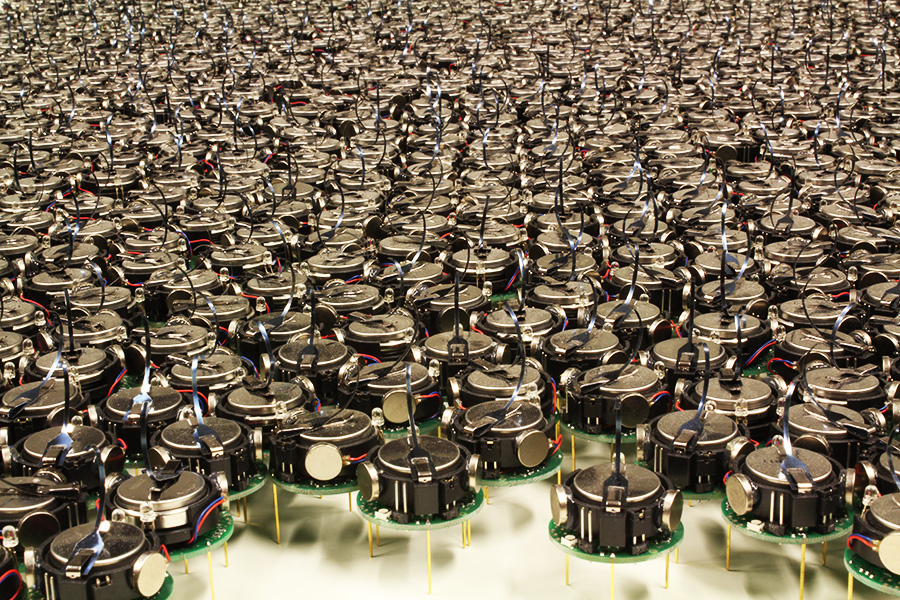
\includegraphics[width=0.3\textwidth]{img/swarms.jpg}
      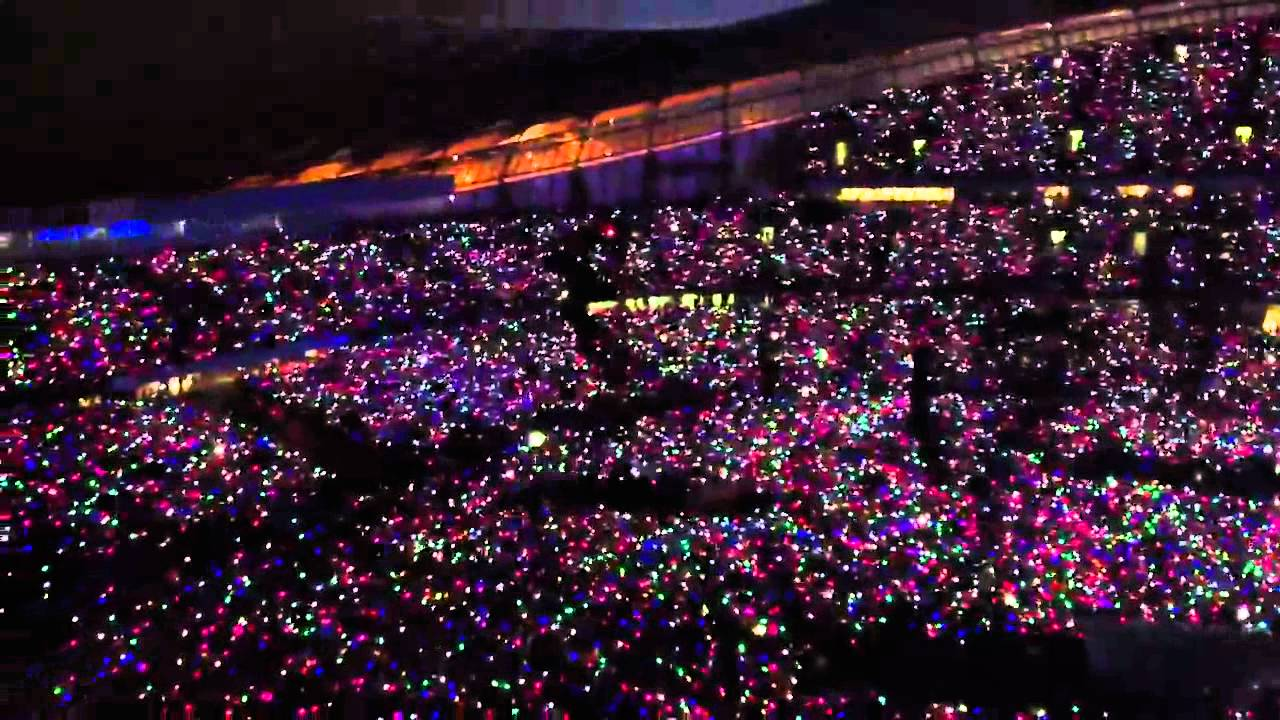
\includegraphics[width=0.3\textwidth]{img/coldplay.jpg}
      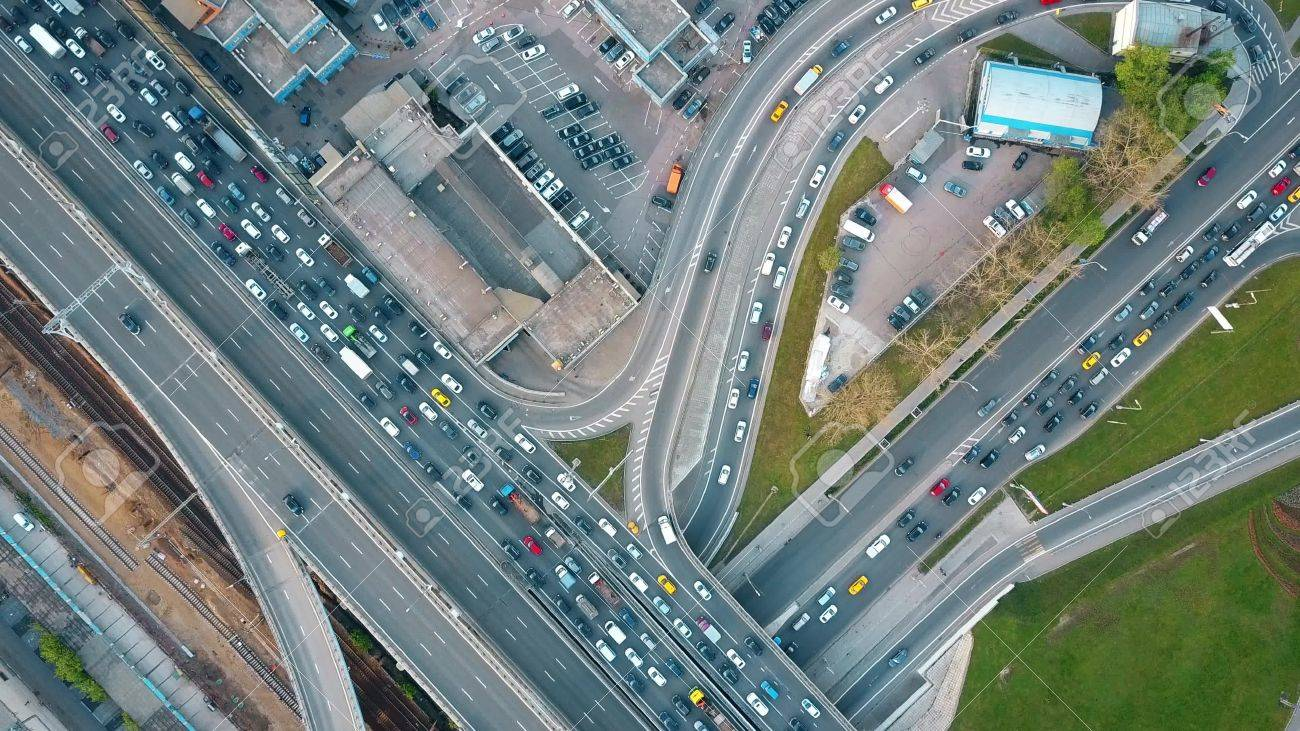
\includegraphics[width=0.3\textwidth]{img/traffic.jpg} 
      %\caption{Examples of Cyber-Physical Swarms}
  \end{figure}
  \end{center}
\end{frame}
\begin{frame}{Context -- Cont.}
\begin{alertblock}{Applications}
  \begin{multicols}{3}
    \begin{itemize}
      \item Swarm robotics
      \item Crowd of (augmented) people
      \item Large-scale IoT systems
      \item Smart cities
      \item COMMunity-OrieNted WEARrable Computing Systems (PRIN project)
    \end{itemize}
  \end{multicols}
\end{alertblock}

\begin{block}{Challenges}
  \begin{multicols}{3}
    \begin{itemize}
      \item (Unwanted) emergents
      \item Local to global mapping
      \item Scale
      \item Failures
      \item Distributed control
      \item Complex \& layered architectures
    \end{itemize}
  \end{multicols}
\end{block}
\begin{center}
  \Large{How can we \bold{engineer} such systems?}
  \end{center}
  \begin{center}
    \Large{What are the right \bold{abstractions}?}
  \end{center}
  \begin{center}
    \Large{This thesis focuses on these questions!}
  \end{center}
\centering
\end{frame}
\begin{frame}{Thesis Goal}
  \begin{alertblock}{Thesis Goal}
    %Devise methodologies and practices to \textbf{synthesize} and \textbf{deploy} \emph{\underline{self-organizing}} behaviors with \textbf{predictable} outcomes.
    Develop a software engineering framework for CPSWs, 
    incorporating \emph{manual} and \emph{automatic} techniques to enable the \underline{design}, \underline{synthesis}, and \underline{deployment} of \emph{self-organizing} behaviors with \emph{scalable} and \emph{robust} outcomes.
  \end{alertblock}

  \begin{exampleblock}{Multi-Faceted Scientific Problem}
    \begin{itemize}
      \item \textbf{How} to express collective behaviors (algorithms \& methodologies)
      \item \textbf{How} to execute specific behaviors (execution models \& middleware dynamics)
      \item \textbf{How} to deploy the computation \emph{\underline{smartly}} (deployment) 
    \end{itemize}
  \end{exampleblock}
\end{frame}

\begin{frame}{State-of-the-art}

  \begin{exampleblock}{Manual Design}
    Approaches in which the collective behavior is \emph{\underline{manually}} designed:
    \begin{itemize}
      \item Finite state machines, rule-based systems, etc.
        \begin{itemize}
          \item Bottom-up, high knowledge requirements, and the collective behavior emerges.
        \end{itemize}
      \item Programming languages with primitives and \emph{collective} abstractions for CPSW (macroprogramming):
        \begin{itemize}
          \item Buzz: a language for programming swarms of drones.
          \item \textbf{Aggregate computing}: a language for programming collective behaviors based on computational fields.
        \end{itemize}
    \end{itemize}  
  \end{exampleblock}

  \begin{exampleblock}{Automatic Design}
    \begin{itemize}
      \item Genetic algorithms, evolutionary strategies, etc.
        \begin{itemize}
          \item \emph{\underline{Black-box}} approach, not predictable, hard to scale up in complexity.
        \end{itemize}
      \item Single-agent machine learning (e.g., reinforcement learning):
        \begin{itemize}
          \item \emph{\underline{Single-agent}} not suitable for collective behaviors (i.e., uncontrolled emergents).
        \end{itemize}
      \item \textbf{Many-agent reinforcement learning}: a way to learn collective behaviors with a large population of agents.
    \end{itemize}
  \end{exampleblock}
\end{frame}

\begin{frame}[plain]
\begin{center}
\Huge{\bold{Aggregate Computing}}
\end{center}
\centering
\large{Program the aggregate, not the individual}
\\ \vspace{0.5cm}
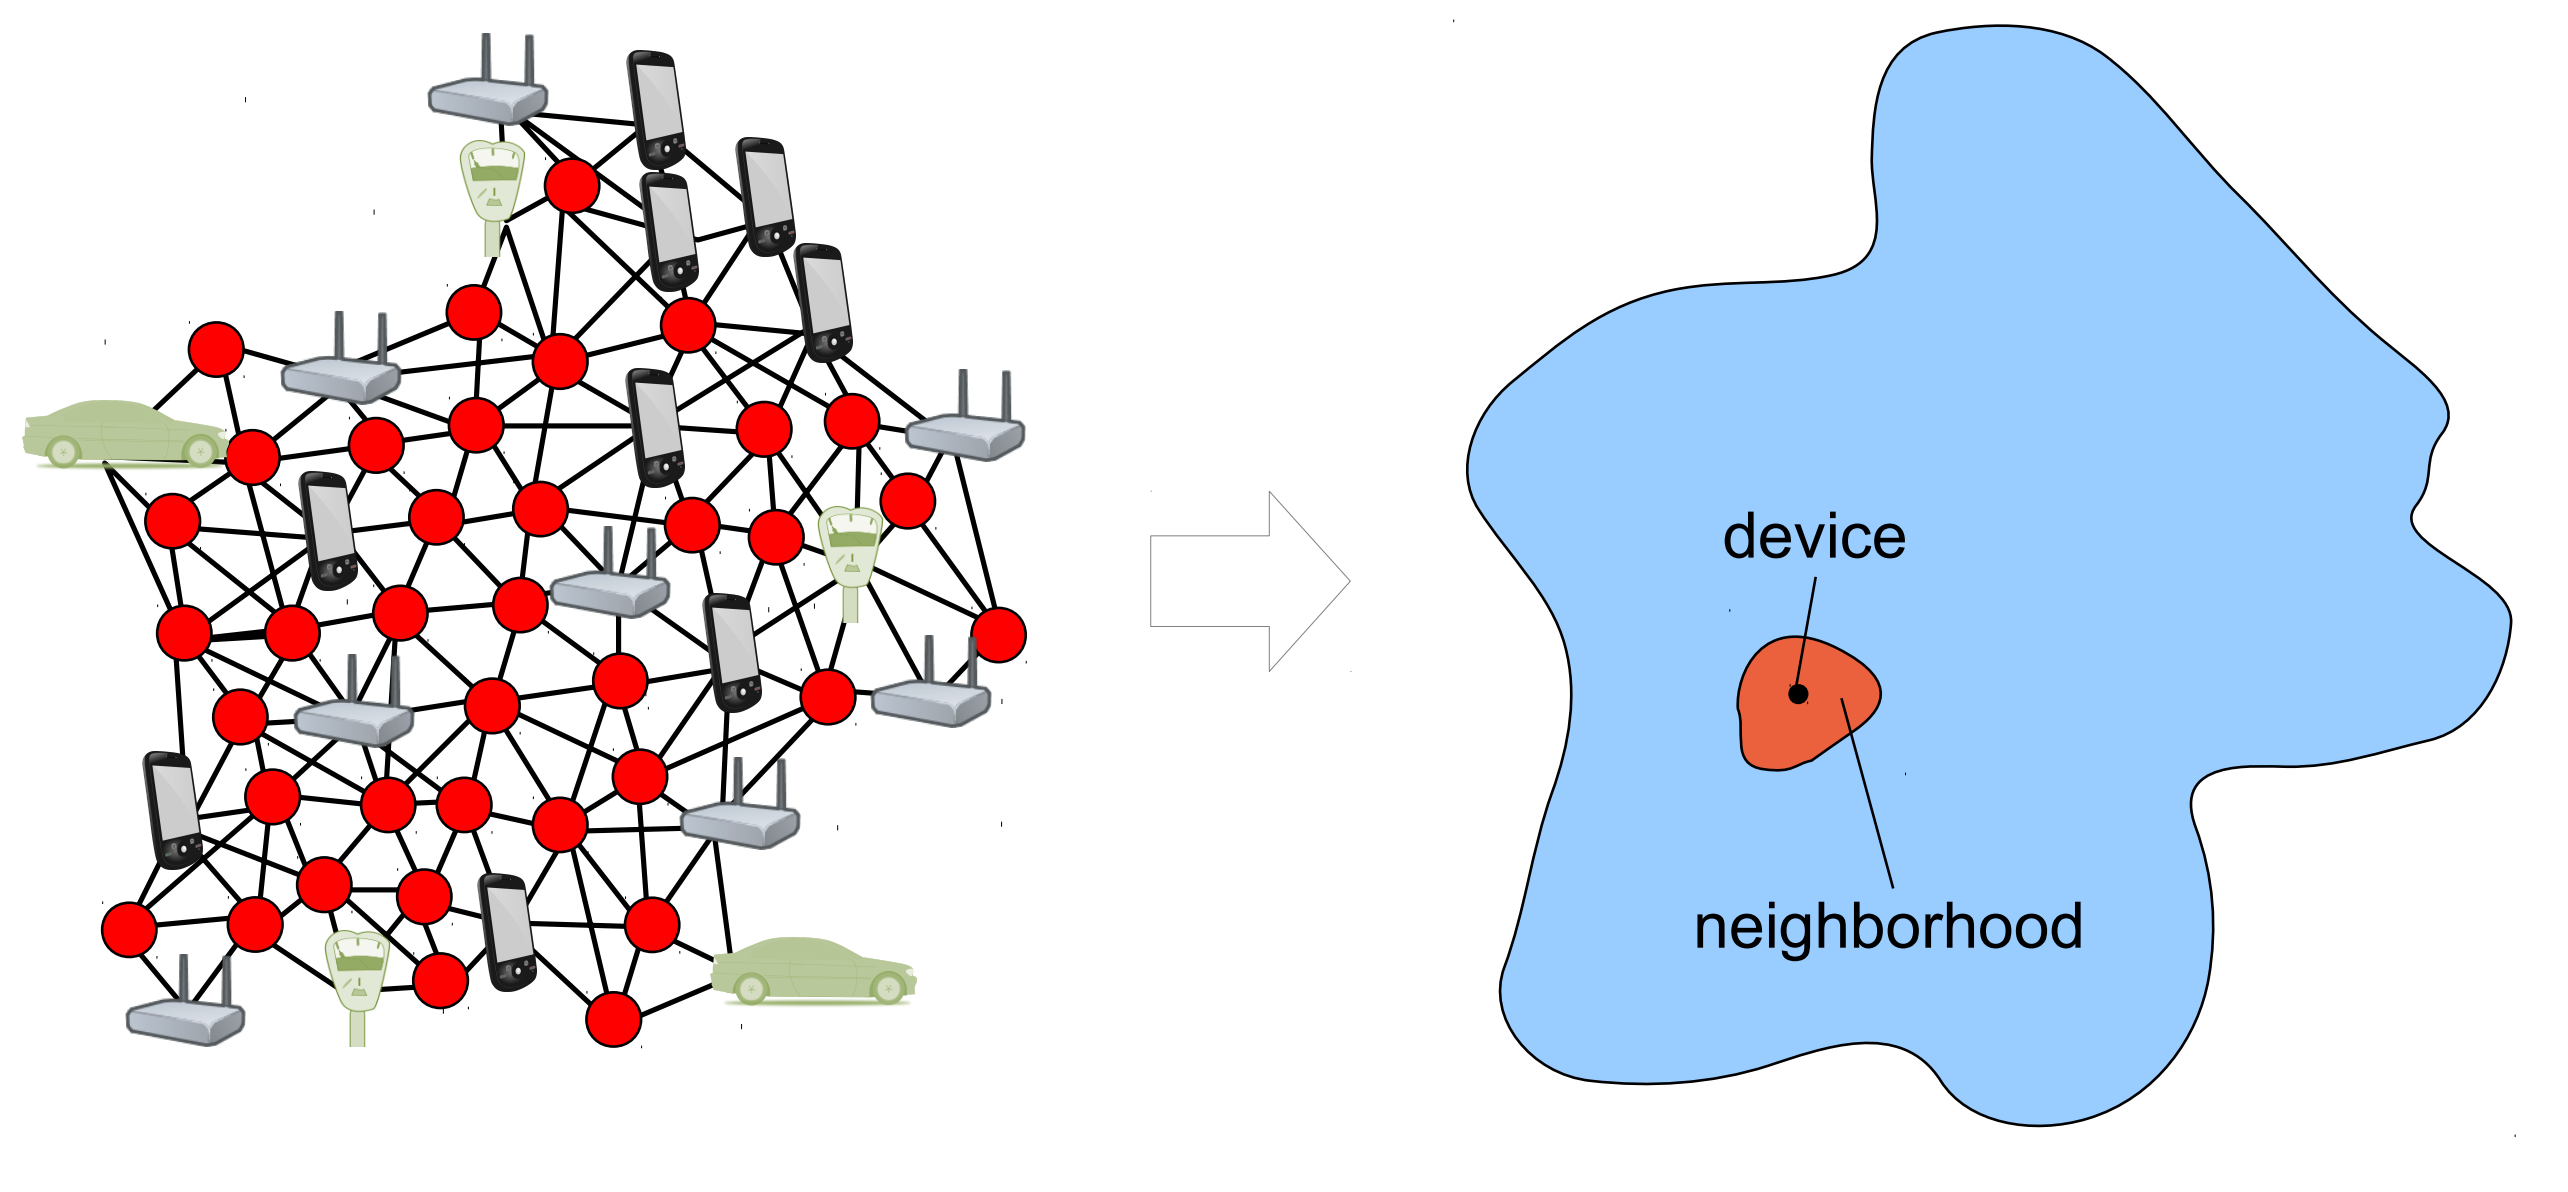
\includegraphics[width=0.8\textwidth]{img/ac.png}
\end{frame}
\begin{frame}{Aggregate Computing -- One slide}
  \hsplit{

  \begin{block}{\footnotesize Self-org-like computational model}
  \scriptsize
  
  \lbl{interaction:} \emph{repeated} msg exchange with \bo{neighbors}\vspace{0.1cm}
  
  \lbl{behavior:} \emph{repeated} execution of \enf{async rounds} of \bo{sense -- compute -- (inter)act} \vspace{0.1cm}
  
  
  \lbl{formal model of executions:} event structures \vspace{0.1cm}
  
  \end{block}
  
  \begin{block}{}
  \scriptsize
  
  \lbl{formal core language:} field calculus~\cite{vbdacp:ac:survey:jlamp}\vspace{0.1cm}
  
  \lbl{paradigm:} \bo{functional, macro-programming} \vspace{0.1cm} %--- supporting compositionality
  
  \centering
  \imgv{0.22}{channel.pdf}
  \end{block}
  
  }{
  \begin{block}{\footnotesize Why?}
    \scriptsize
    
    {\bold{\faThumbsUp}} \, Decouple the collective specification from the IT networks  \vspace{0.1cm}
    
    {\bold{\faThumbsUp}} \, Scale naturally with nodes in the systems  \vspace{0.1cm}
     
    {\bold{\faThumbsUp}} \, High-level abstractions to devise applications
    
    %\lbl{semantics:} (1) device; (2) network; (3) global comp.
  \end{block}
  %}
  
  \begin{block}{} %{Engineering approach}
    \scriptsize
  \lbl{abstraction:} \bo{computational fields} ($\mathit{dev/evt} \mapsto \mathbb{V}$) \vspace{0.1cm}
    \lbl{examples:} \bo{temperature fields}, \bo{actuation fields} \vspace{0.1cm}
    \begin{center}
      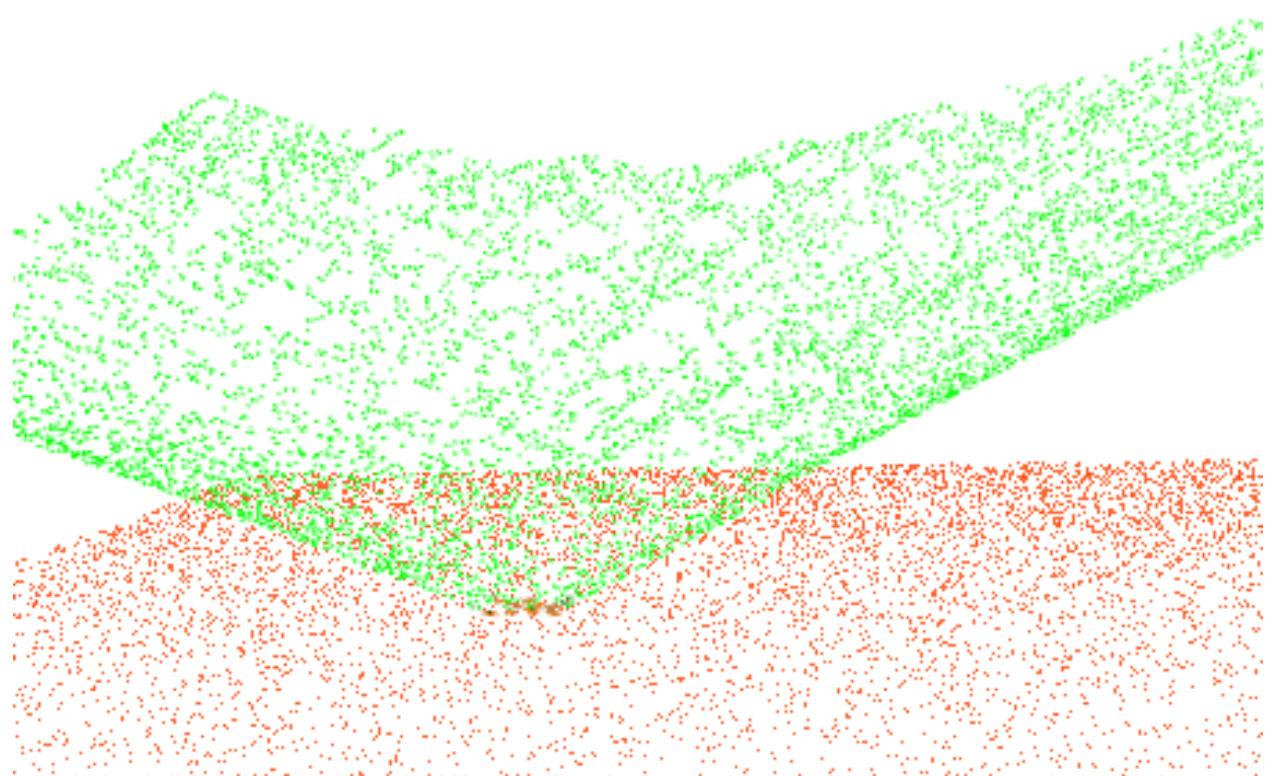
\includegraphics[width=0.3\textwidth]{img/3d-gradient.png}
      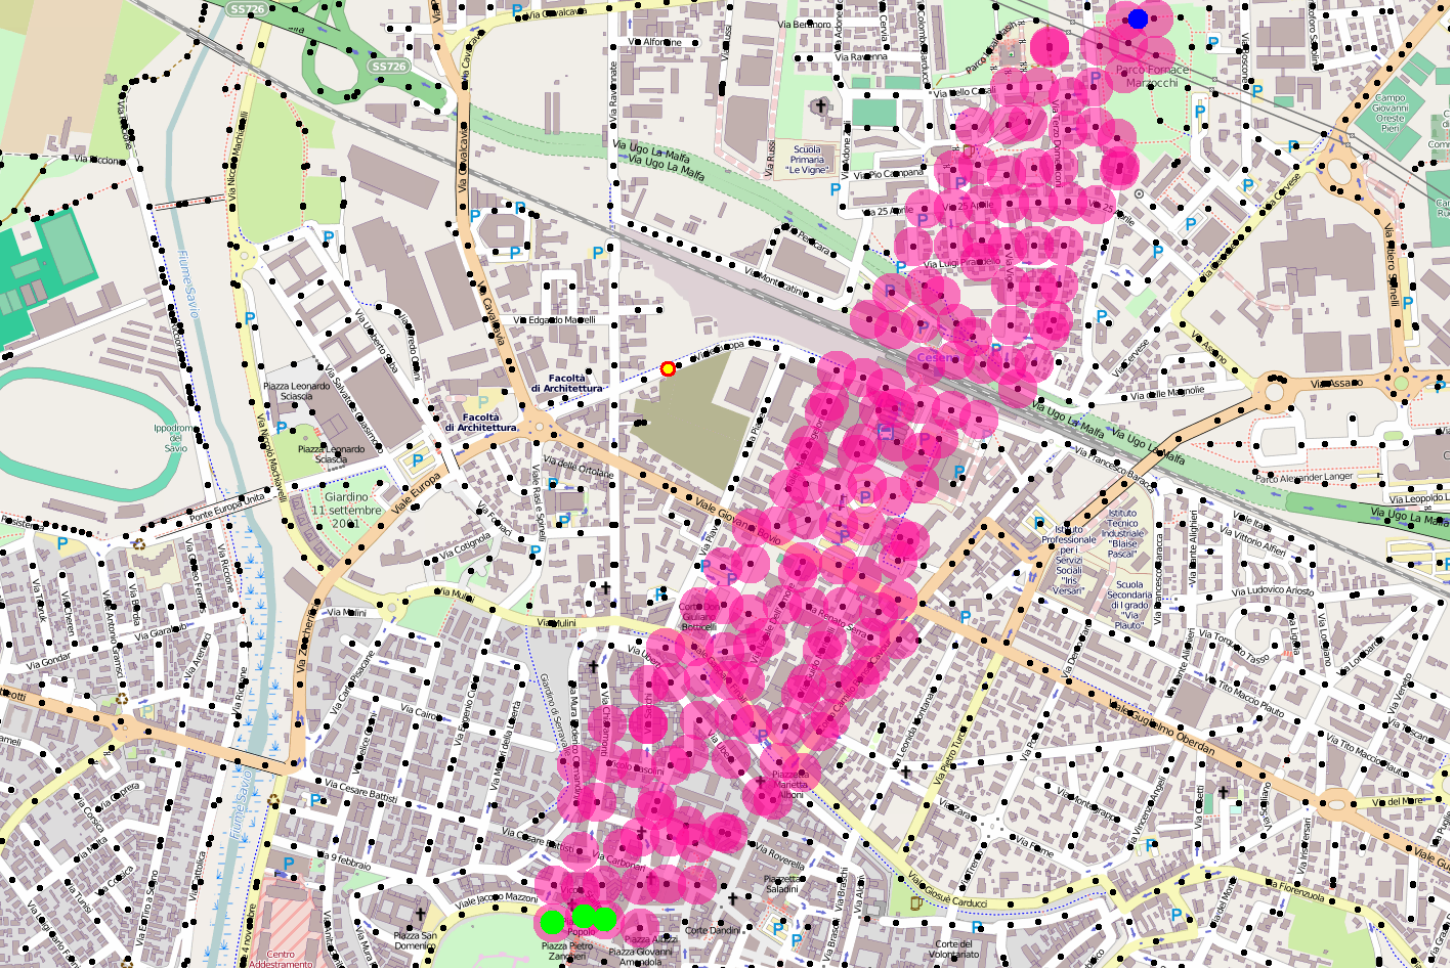
\includegraphics[width=0.28\textwidth]{img/channel.png}
      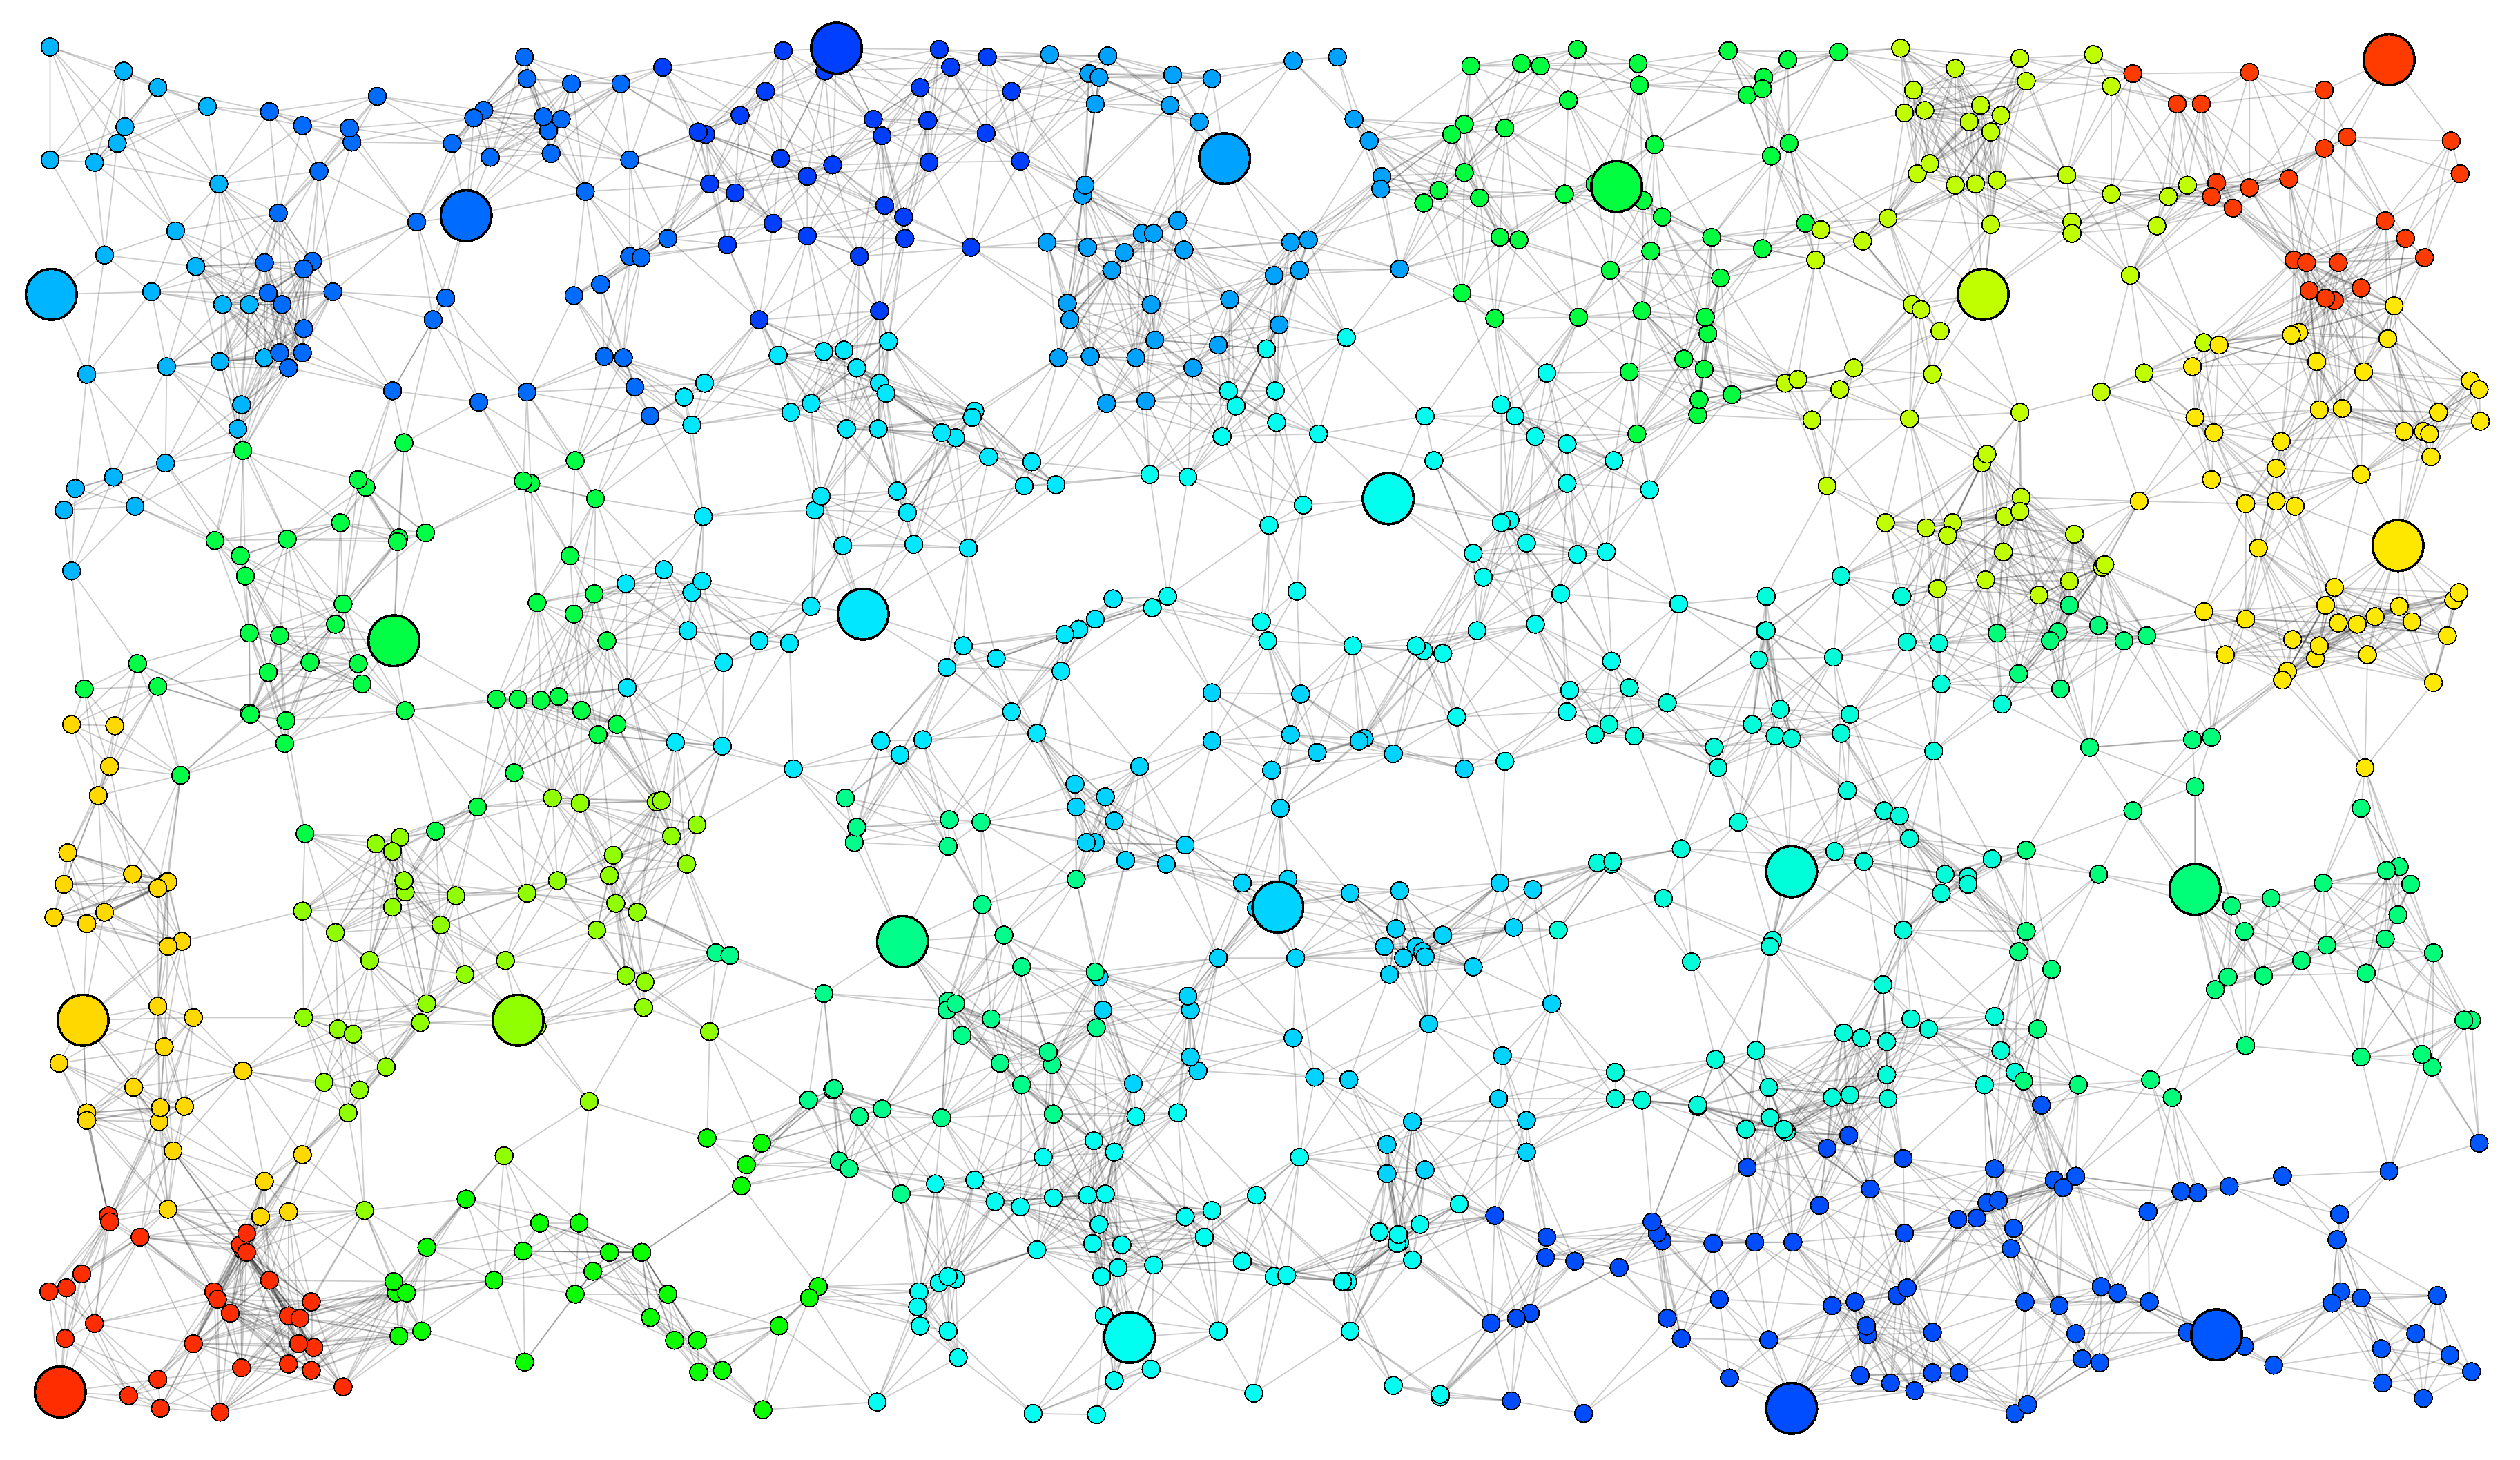
\includegraphics[width=0.3\textwidth]{img/scr-result.png}
      \end{center}
  \tiny \fullcite{bpv:aggregate:programming}
  \end{block}
  %}
  }
  
\end{frame}

\begin{frame}[plain]
  \begin{center}
\huge{\bold{Many-agent Reinforcement Learning}\footnote{\tiny\fullcite{yang2021many}}}\footnote{\tiny\fullcite{DBLP:journals/corr/abs-2209-03859}}
  \end{center}
  \begin{center}
    \large{A multi-agent learning environment in which a \bold{large} group agents learn to \bold{coordinate} their actions to achieve a \emph{\underline{collective}} goal}.
  \end{center}
\end{frame} 
\begin{frame}{Many-agent Reinforcement Learning}

\begin{alertblock}{A Tentative Formal Model: SwarMDP~\cite{vsovsic2016inverse}}
    SwarMDP is a formal model composed of a \emph{swarming agent} $\mathbb{A}$ and an \emph{environment} $\mathbb{E}$:
    \begin{itemize}
      \item Agent $\mathbb{A}$: Has observation and action spaces, a reward signal, and a policy.
      \item Environment $\mathbb{E}$: Has a state space, a population of swarming agents, a transition function, and a global reward function.
      \item System Evolution: Evolves in discrete time steps, where agents $\mathbb{A}$ interact with the environment $\mathbb{E}$ by executing actions and receiving rewards.
      \item \textbf{Goal}: Learn a policy $\pi$ that maximizes the \textbf{expected return}.
    \end{itemize}
\end{alertblock}

\begin{block}{Learning in SwarMDP}
  \begin{itemize}
    \item SwarMDP \faArrowRight \, large-scale handling via a \textbf{homogeneous} policy:
      \begin{itemize}
        \item The same policy is shared within the population.
      \end{itemize}
    \item Learning: \emph{centralized}, but execution is \textbf{decentralized}.
    \item Algorithms:
      \begin{itemize}
        \item \underline{Mean-field RL \cite{yang2018mean}}: Learning by considering neighboring agents as an approximation of the global state.
        \item \underline{Swarm RL \cite{iima2008swarm}}: A way to learn the Q-function in a swarm of agents.
      \end{itemize}
  \end{itemize}
\end{block}

\end{frame}

\begin{frame}{Going Beyond the State-of-the-Art}

  \begin{alertblock}{Engineering Perspective}
    \begin{itemize}
        \item \emph{API Design}: Bridge the gap between AC and real-world applications.
        \item \emph{Programming Model}: Develop an intuitive way to express collective behaviors.
        \item \emph{Intelligent Deployment}: Optimize the deployment of aggregate programs across diverse infrastructures, enhancing adaptability and efficiency.
        \item \emph{Practical Tooling}: Create user-friendly tools for prototyping and deploying aggregate programs, fostering broader adoption.
        \item \textbf{\underline{Key Motivation}}: Aggregate computing requires refined abstractions and tools to effectively engineer the complex world of CPSWs.
    \end{itemize}
  \end{alertblock}

  \begin{alertblock}{Learning Perspective}
    \begin{itemize}
        \item \emph{AC for Learning}: Utilize aggregate computing to build robust and resilient learning infrastructures, e.g., for federated learning or multi-agent RL.
        \item \emph{Learning for AC}: Leverage machine learning techniques to dynamically optimize and adapt the aggregate computing model itself.
        \item \textbf{\underline{Key Motivation}}: Learning is essential to adapt aggregate computing to the highly dynamic and complex nature of real-world environments.
    \end{itemize}
  \end{alertblock}

\end{frame}

\begin{frame}{Contribution -- One slide}
\centering{\huge{\textbf{\underline{Language-based} software engineering for CPSWs}}}
\\[0.5cm]
%\begin{center}

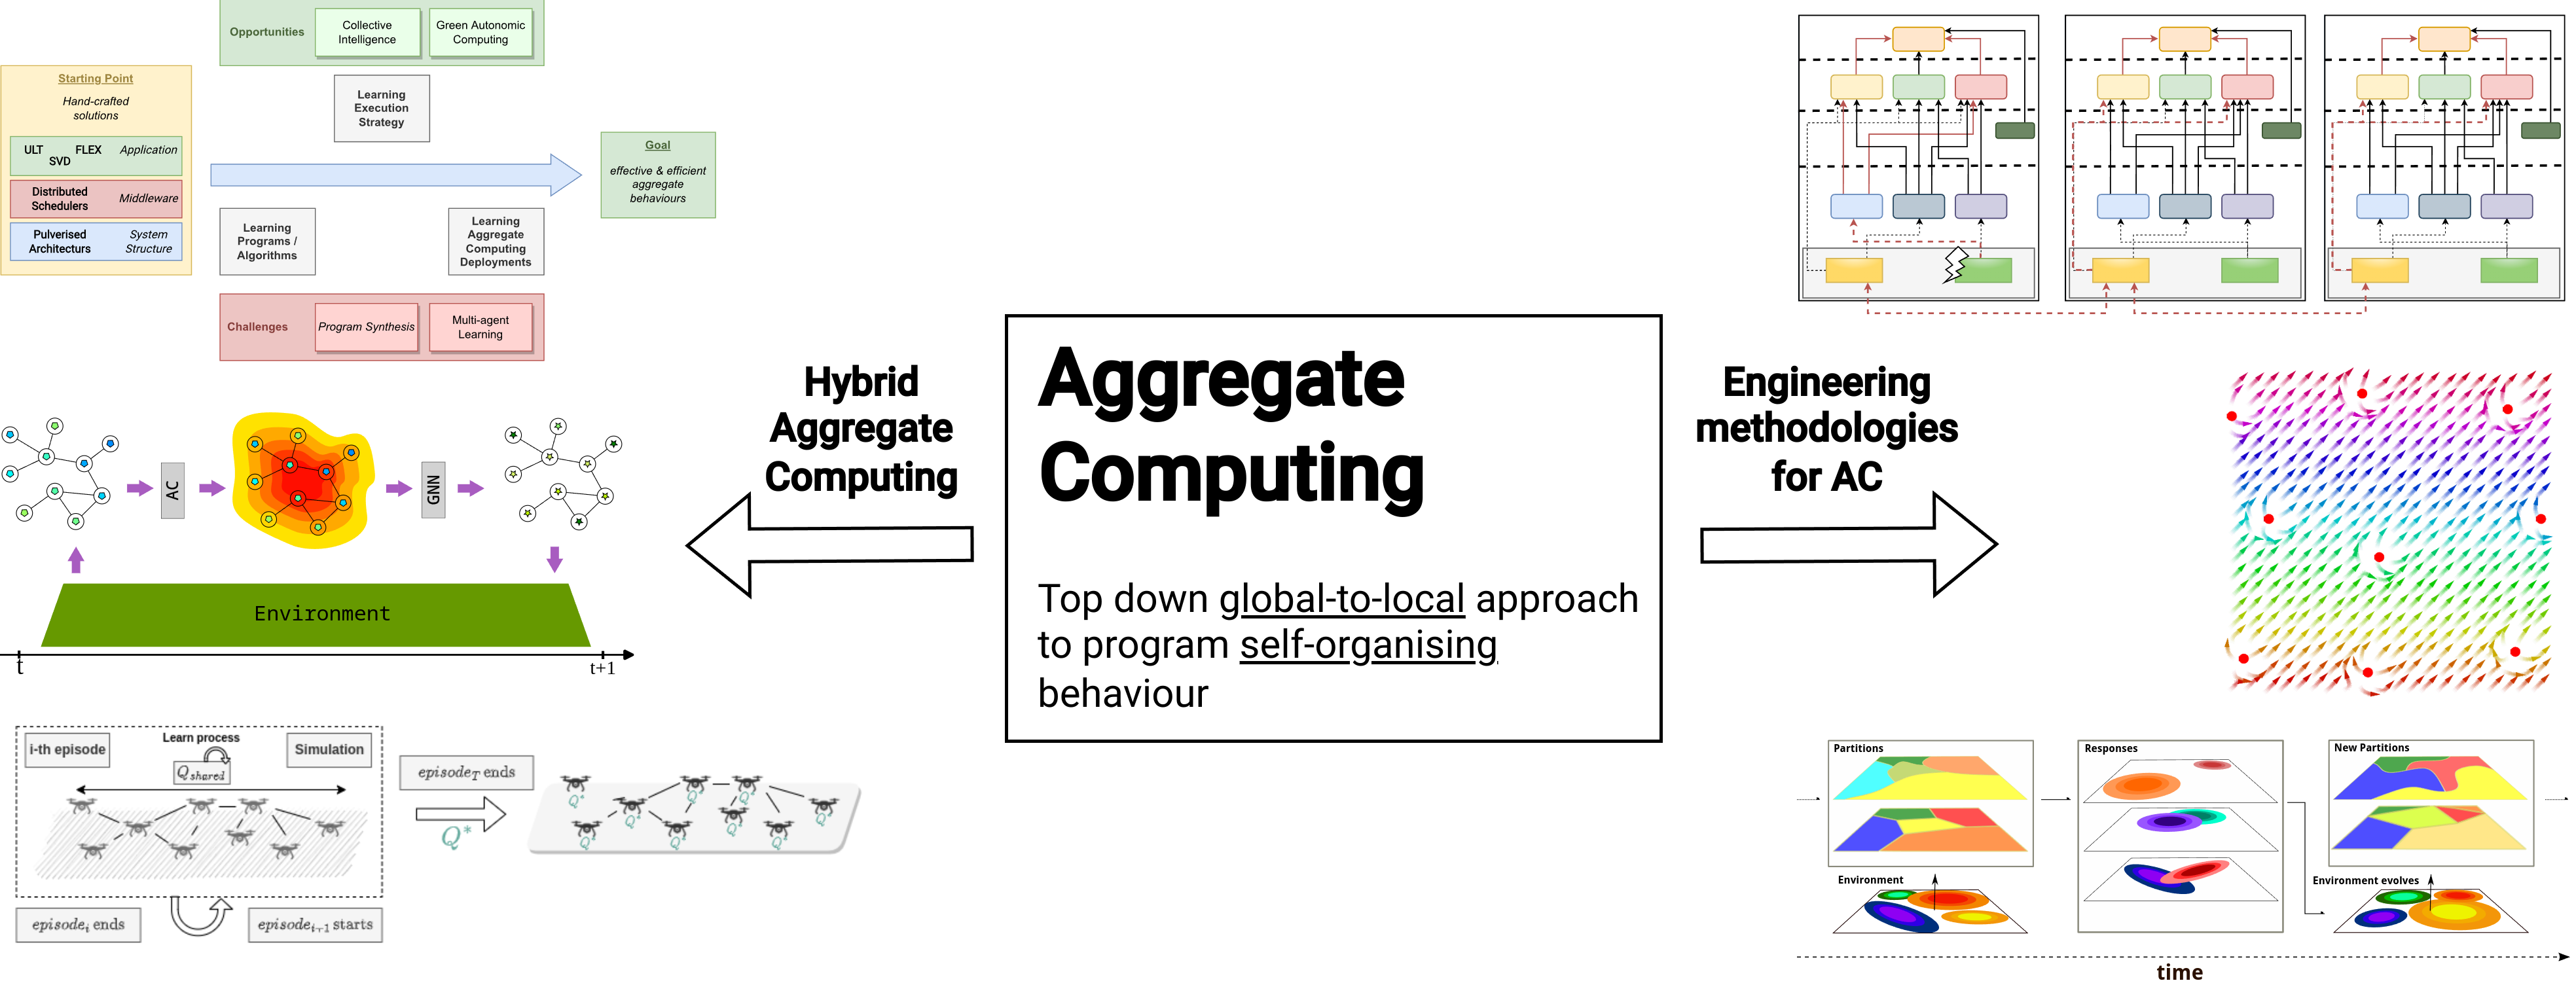
\includegraphics[width=\textwidth]{img/contribution.drawio.png}
%\fbox{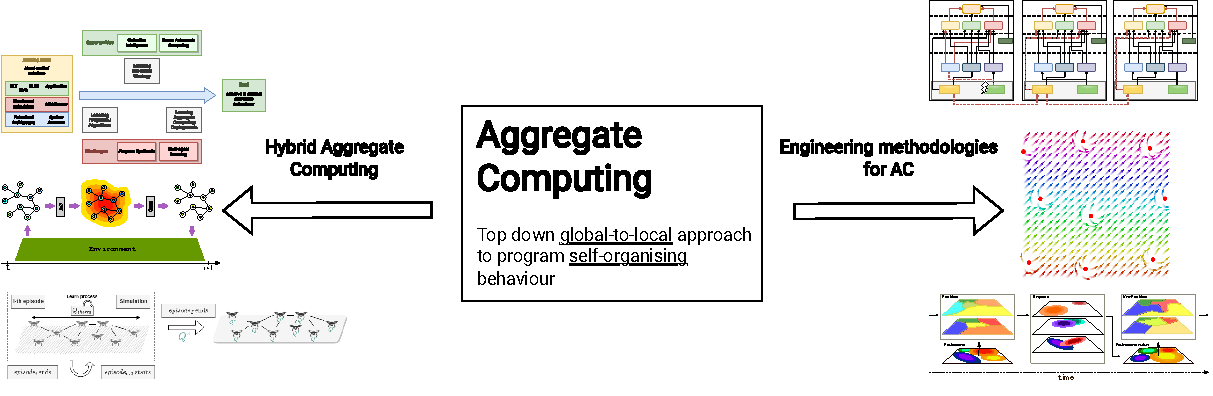
\includegraphics[width=0.95\textwidth]{img/contribution.drawio.pdf}}
%\end{center}
\end{frame}
\begin{frame}{Hybrid Aggregate Computing}

  \textbf{Areas of Improvement:}
  
  \begin{enumerate}
  \item \textbf{Execution Policies for Efficiency:}
      \begin{itemize}
      \item \textbf{Adaptive Collective Schedulers~\cite{DBLP:conf/acsos/AguzziCV22}:} Shared-experience Q-learning to dynamically optimize execution for convergence speed or resource consumption.
      \item \textbf{Self-Stabilizing Systems:} Focus on reducing consumption while maintaining the self-healing properties of collectives.
      \end{itemize}
  \item \textbf{Collective Program Synthesis:}
      \begin{itemize}
      \item \textbf{Program Sketching~\cite{DBLP:conf/coordination/AguzziCV22}:} Q-learning for completing partial programs, tailoring coordination blocks to specific environmental dynamics (e.g., mobility, failures).
      \item \textbf{Goal:} Automate the generation of adaptable blocks, overcoming limitations of heuristic-based approaches.
      \end{itemize}
  \item \textbf{\underline{Many-Agent RL through AC}:}
      \begin{itemize}
      \item \textbf{Field-Informed RL~\cite{acgnn}:} Aggregate information (fields) guides policy learning in complex CPSW environments.
      \item \textbf{Graph Neural Networks:} Leverage graph neural networks for policy approximation, achieving faster and more scalable learning.
      \end{itemize}
  \end{enumerate}
  
\end{frame}
\begin{frame}{AC for Learning: Field-Informed Reinforcement Learning}
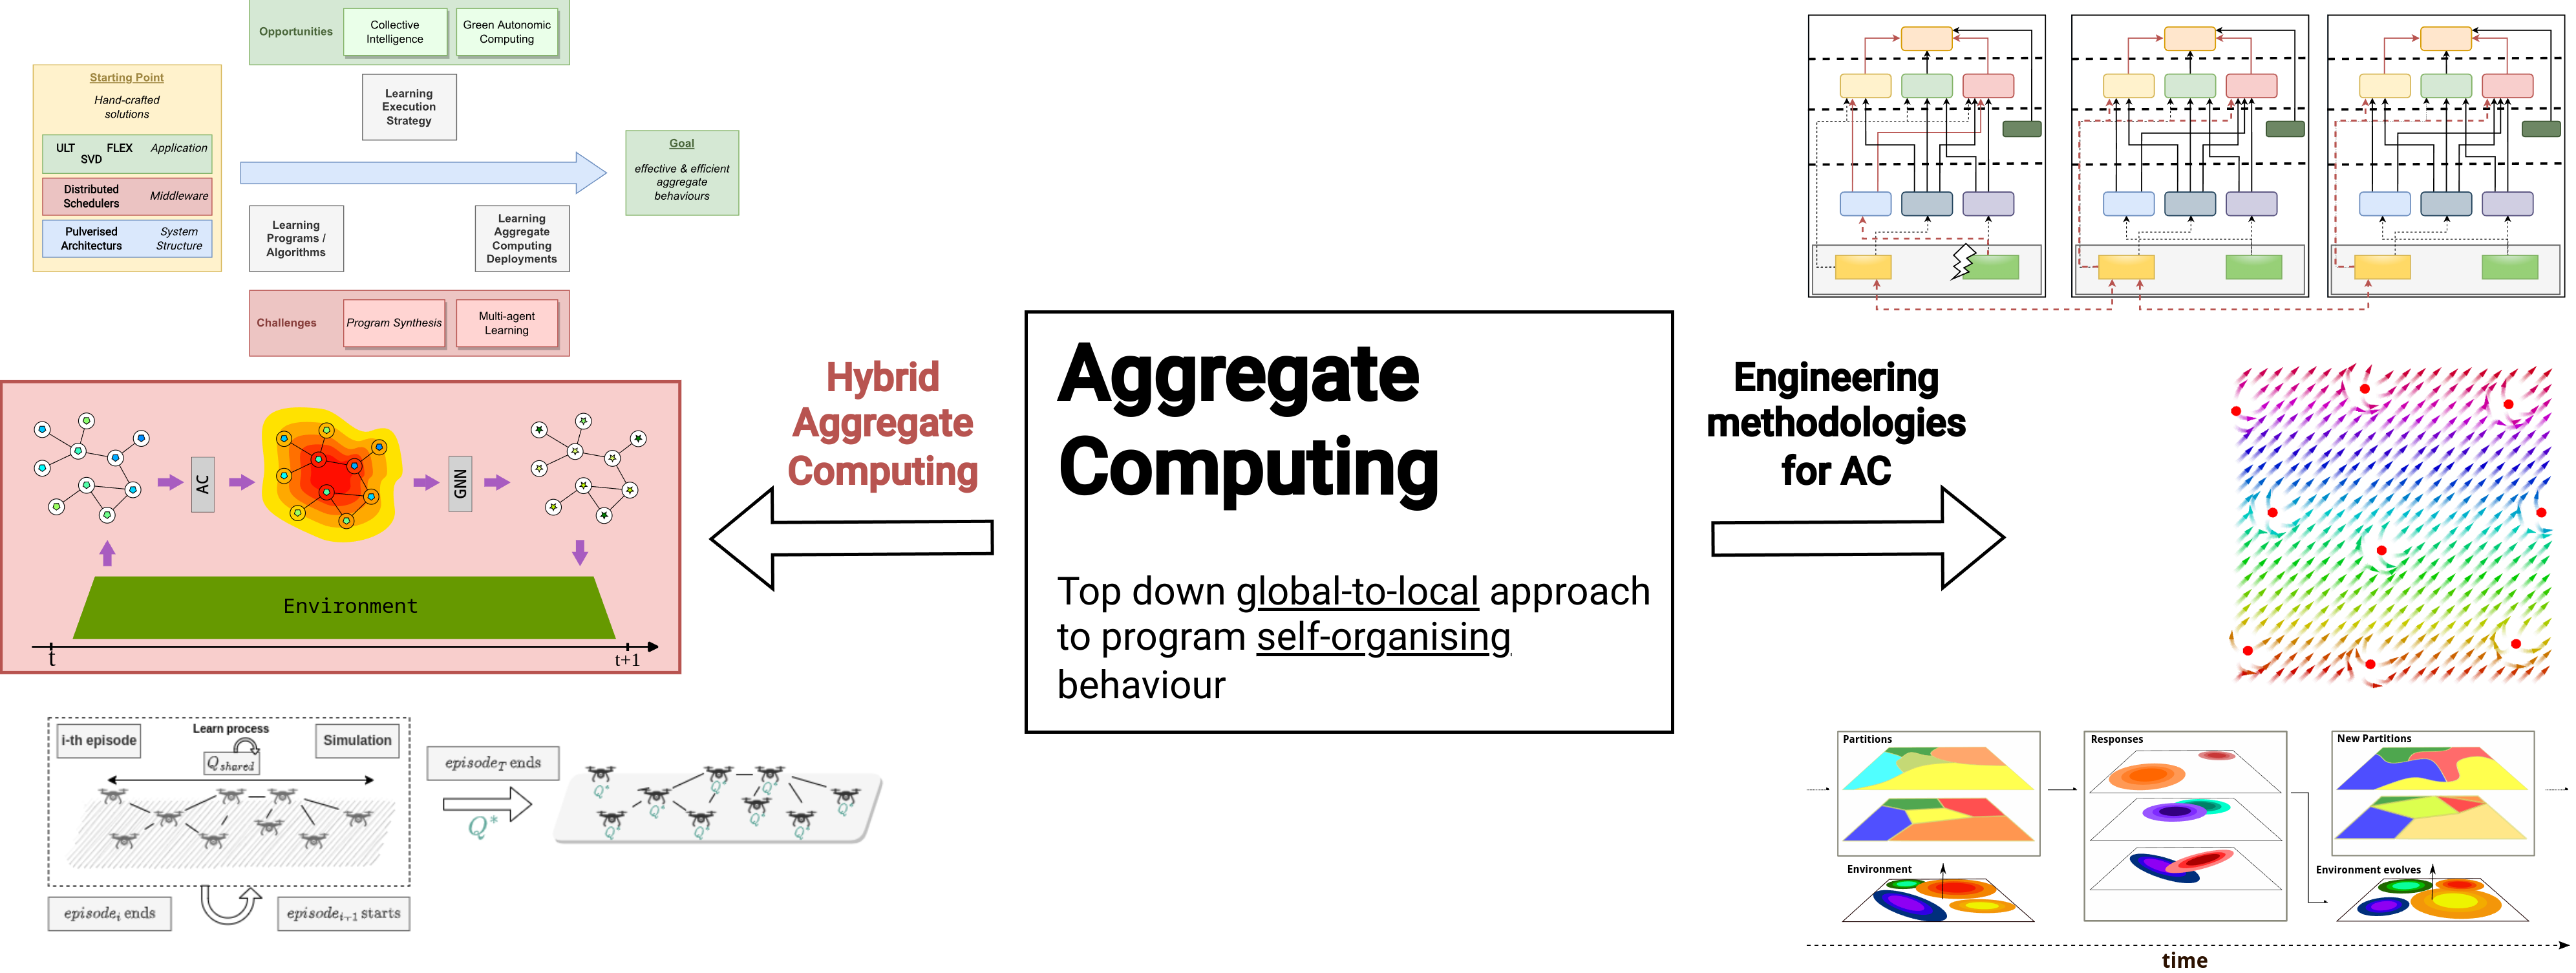
\includegraphics[width=\textwidth]{img/contribution-focus.drawio.png}
\end{frame}
\begin{frame}{AC for Learning: Field-Informed Reinforcement Learning}

  \begin{block}{Problem}
    \begin{itemize}
      \item \textbf{Collective Aspect}: The state typically lacks a global representation \faArrowRight \, \emph{\underline{partial observability}}.
        \begin{itemize}
          \item It is built through communication with neighbors.
        \end{itemize}
      \item \textbf{Variable Neighborhood}: 
        \begin{itemize}
          \item The need for a policy that accounts for neighborhood \emph{\underline{variability}}.
        \end{itemize}
    \end{itemize}
  \end{block}

  \begin{alertblock}{\textbf{Contribution}: Field-Informed Reinforcement Learning\footnote[frame]{\fullcite{acgnn}}} 
    \begin{itemize}
      \item \textbf{Fields}: Used to produce a \emph{\underline{stigmergic}} representation of the environment.
      \begin{itemize}
        \item \textbf{GNN}: Policy function approximator that handles neighborhood variability.
        \item \textbf{Graph-Deep Q Learning}: Learning algorithm.
        \item \textbf{Aggregate Computing}: Informs the learning process with computational fields.
      \end{itemize}
    \end{itemize}
  \end{alertblock}

\end{frame}
\begin{frame}{FIRL: Graph Neural Networks}
  \begin{exampleblock}{What}
    A neural network architecture designed to work with graph-structured data.
  \end{exampleblock}

  \begin{center}
    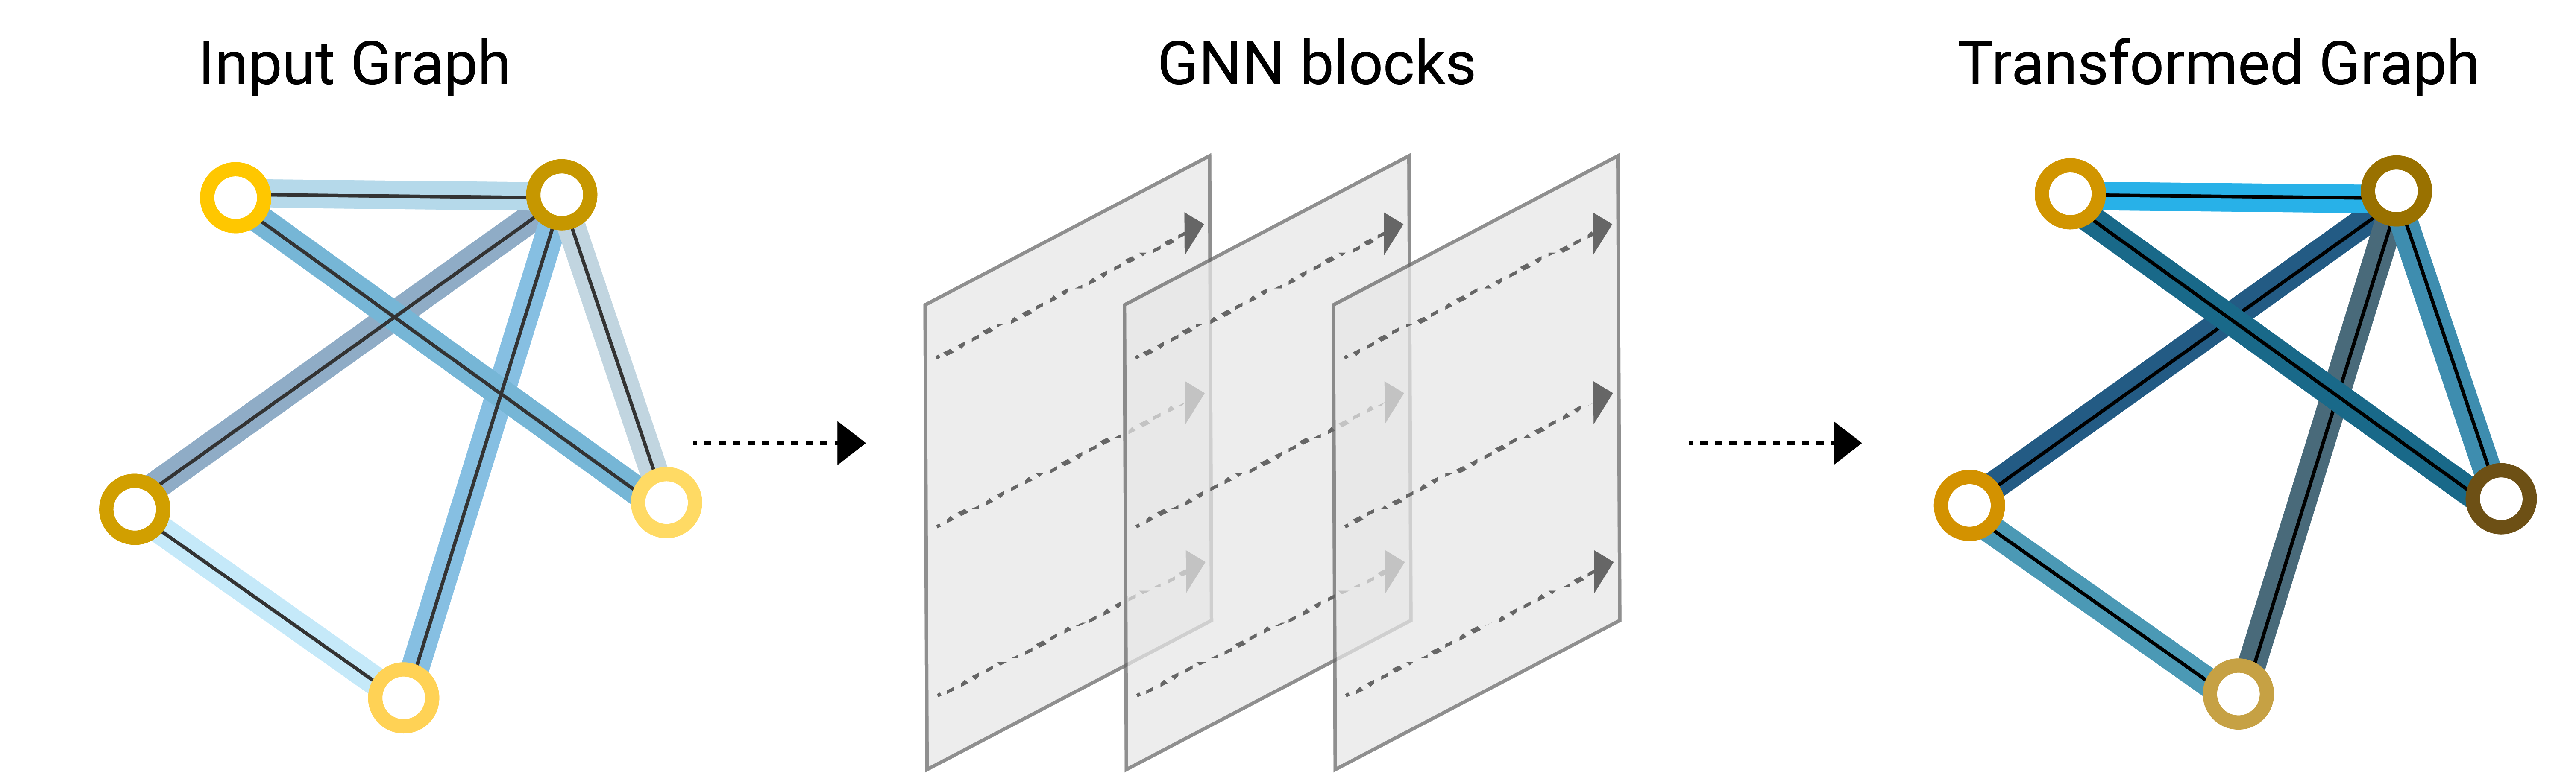
\includegraphics[width=0.5\textwidth]{img/gnn.png}
  \end{center}

  \begin{block}{How}
    \begin{itemize}
      \item \textbf{Message Passing:} Update node representations based on their neighborhood.
      \item \textbf{Aggregation:} Combine information from neighboring nodes.
      \item \textbf{Update:} Modify node representations based on the aggregated information.
    \end{itemize}
  \end{block}

  \begin{alertblock}{Why}
    \begin{itemize}
      \item \textbf{Dual Interpretation:} Offers both global and local perspectives on graph data.
      \item \textbf{Handles Variability:} Effectively addresses the varying structure and size of neighborhoods in graphs.
    \end{itemize}
  \end{alertblock}
\end{frame}

\begin{frame}{FIRL: Graph-Deep Q Learning}
  \begin{block}{What}
    A learning algorithm which uses GNN as a policy function approximator
  \end{block}
  \begin{block}{How}
    \begin{itemize}
      \item \bold{Graph Experience replay}: store the experience in a replay buffer under the form of graphs
      \item \bold{Target network}: use a target network to stabilize the learning and using GNNs
    \end{itemize}
  \end{block}
  \begin{alertblock}{Why}
    \begin{itemize}
      \item Handle many-agent through shared experience pattern 
      \item Follow a centralized learning approach but with a decentralized execution (thanks to GNN)
    \end{itemize}
  \end{alertblock}
\end{frame}
\begin{frame}{FIRL: Overall learning step}
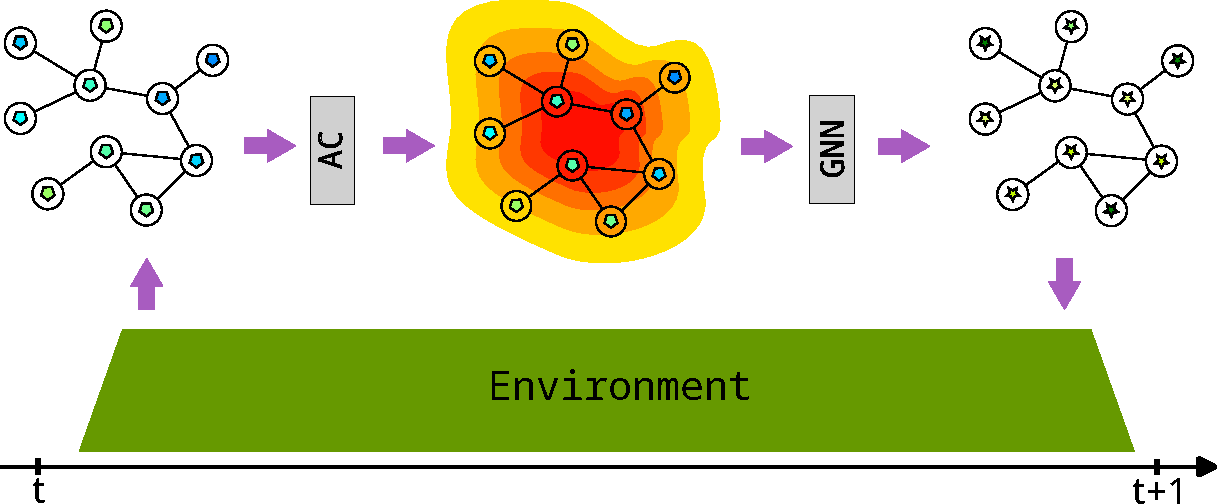
\includegraphics[width=\textwidth]{img/architecture.pdf}
\end{frame}
\begin{frame}{FIRL: Algorithm}
  \begin{algorithm}[H]
    \KwIn{Environment $\mathbb{E}$, Graph Replay $\mathcal{D}$, Target Network $\theta^-$, Current Network $\theta$, Exploration $\epsilon$}
    \KwOut{Trained DQN $\theta$}
    Initialize $\mathcal{D}$, $\theta$, $\theta^- \leftarrow \theta$\;
    \While{not done}{
        Observe $G_o$\;
        $a \leftarrow \begin{cases}
            \text{random action} & \text{if random } < \epsilon \\
            argmax_{a_v} Q(G_o, \theta)[v](a_v) & \text{otherwise}
        \end{cases}$\;
        Execute $a$, observe $G_r$, $G_o'$\;
        Store $(G_o, a, G_r, G_o')$ in $\mathcal{D}$\;
        Sample batch $(G_o^b, a^b, G_r^b, G_o'^b)$ from $\mathcal{D}$\;
        $y_v \leftarrow G_r^b[v] + \gamma \max_{a'} Q(G_o'^b[v], a'; \theta^-)$\;
        $y_v^* \leftarrow Q(G_o^b[v], a^b[v]; \theta)$\;
        $\theta \leftarrow \theta - \alpha \nabla_\theta \frac{1}{|G^b|} (y - y^*)^2$\;
        \If{C steps}{ $\theta^- \leftarrow \theta$ }
    }
    \end{algorithm}
\end{frame}
\begin{frame}{FIRL: Simulation Setup}

  \begin{columns}
    \begin{column}{0.5\textwidth}  % Adjusted width 
        \begin{itemize}
          \item \textbf{Setup}: Group of nodes in a 2D space, neighborhood based on spatial proximity.
          \item \textbf{Goal}: Maximize the coverage of a spatial phenomenon (fire, pollution, etc.).
          \item \textbf{Rewards}: 
            \begin{itemize}
              \item \emph{Inside Phenomenon}: Maximize the number of nodes inside the phenomenon.
              \item \emph{Cohesion}: Minimize the number of isolated nodes.
              \item \emph{Coverage}: Maximize the intersection of covered areas.
            \end{itemize}
          \item \textbf{States}: Relative position of nodes and potential field of the phenomenon.
        \end{itemize}
    \end{column}
    \begin{column}{0.5\textwidth}  % Adjusted width to match the text column
      \centering
      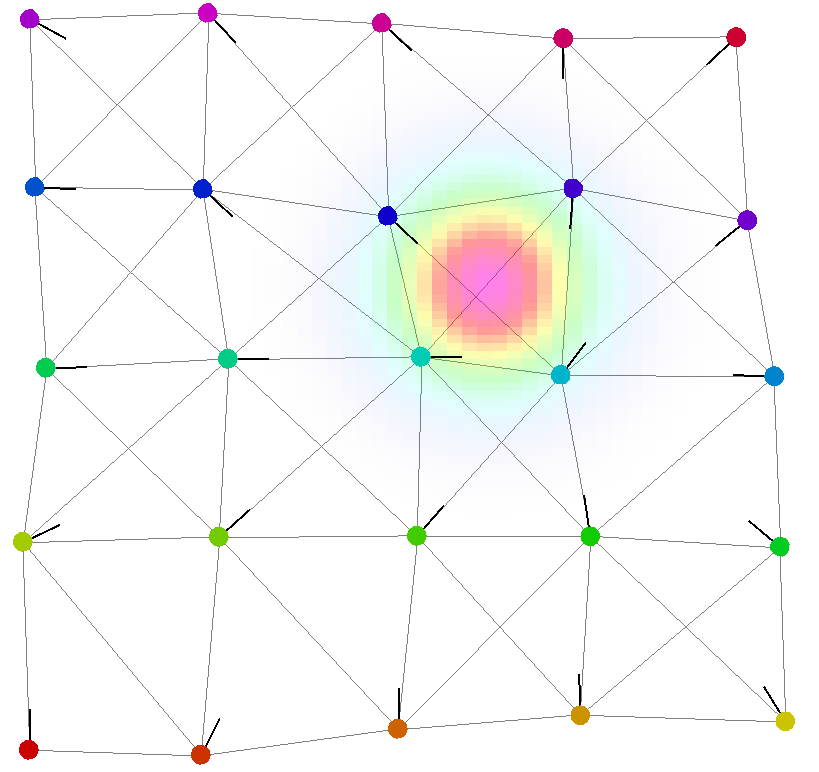
\includegraphics[width=\textwidth]{img/coverage-setup.png}
    \end{column}
  \end{columns}
\end{frame}
\begin{frame}{FIRL: Algorithm}
  \begin{algorithm}[H]
    \KwIn{Environment $\mathbb{E}$, Graph Replay $\mathcal{D}$, Target Network $\theta^-$, Current Network $\theta$, Exploration $\epsilon$}
    \KwOut{Trained DQN $\theta$}
    Initialize $\mathcal{D}$, $\theta$, $\theta^- \leftarrow \theta$\;
    \While{not done}{
        Observe $G_o$\;
        $a \leftarrow \begin{cases}
            \text{random action} & \text{if random } < \epsilon \\
            argmax_{a_v} Q(G_o, \theta)[v](a_v) & \text{otherwise}
        \end{cases}$\;
        Execute $a$, observe $G_r$, $G_o'$\;
        Store $(G_o, a, G_r, G_o')$ in $\mathcal{D}$\;
        Sample batch $(G_o^b, a^b, G_r^b, G_o'^b)$ from $\mathcal{D}$\;
        $y_v \leftarrow G_r^b[v] + \gamma \max_{a'} Q(G_o'^b[v], a'; \theta^-)$\;
        $y_v^* \leftarrow Q(G_o^b[v], a^b[v]; \theta)$\;
        $\theta \leftarrow \theta - \alpha \nabla_\theta \frac{1}{|G^b|} (y - y^*)^2$\;
        \If{C steps}{ $\theta^- \leftarrow \theta$ }
    }
    \end{algorithm}
\end{frame}
\begin{frame}{FIRL: Evaluation}

    Three different scenarios:
    \begin{itemize}
      \item \textbf{Static:} The phenomenon is static.
      \item \textbf{Multiple:} There are multiple phenomena.
      \item \textbf{Dynamic:} The phenomenon is moving.
    \end{itemize}
    \begin{figure}
        \centering
        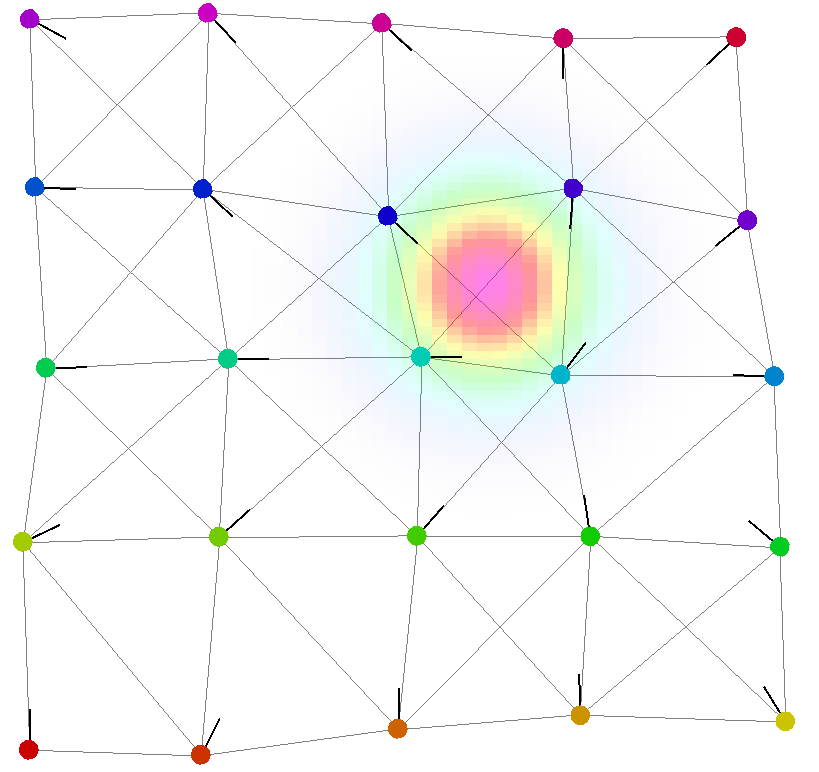
\includegraphics[width=0.15\textwidth]{img/base}
        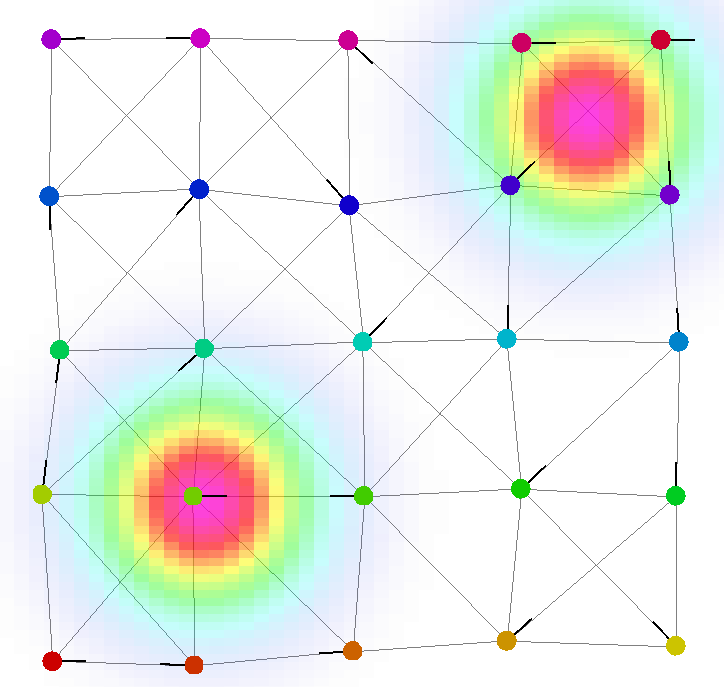
\includegraphics[width=0.15\textwidth]{img/two}
        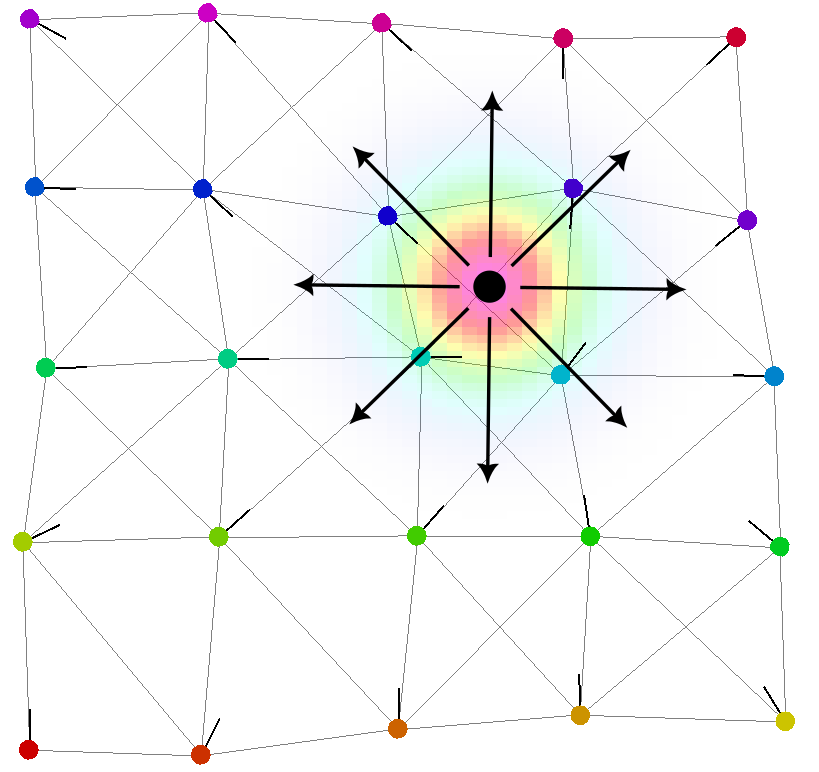
\includegraphics[width=0.15\textwidth]{img/moving}
    \end{figure}

    Under three different solutions:
    \begin{itemize}
      \item \textbf{FIRL:} The proposed solution.
      \item \textbf{Graph Q-learning:} GNN without AC.
      \item \textbf{Deep Q Learning + AC:} MLP with AC.
    \end{itemize}

Evaluation divided into:
  \begin{enumerate}
    \item \textbf{Training Phase:} Performed in the fixed scenario for a total of 2000 steps.
    \item \textbf{Evaluation Phase:} Used all scenarios for 64 different runs.
  \end{enumerate}
\end{frame}

\begin{frame}[allowframebreaks]{FIRL: Results}
  
\begin{center}
  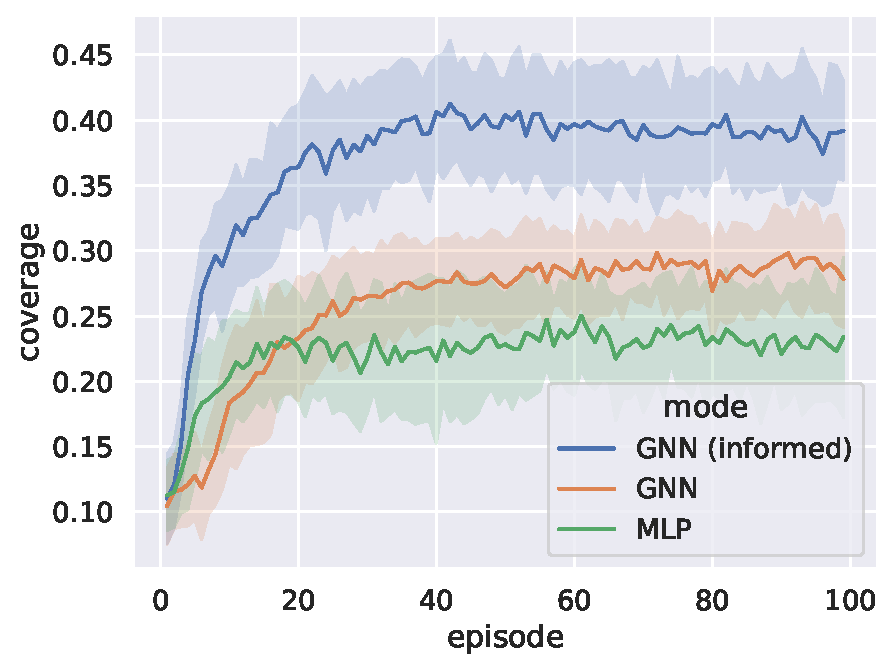
\includegraphics[width=0.35\textwidth]{img/coverage-in-time.pdf}
  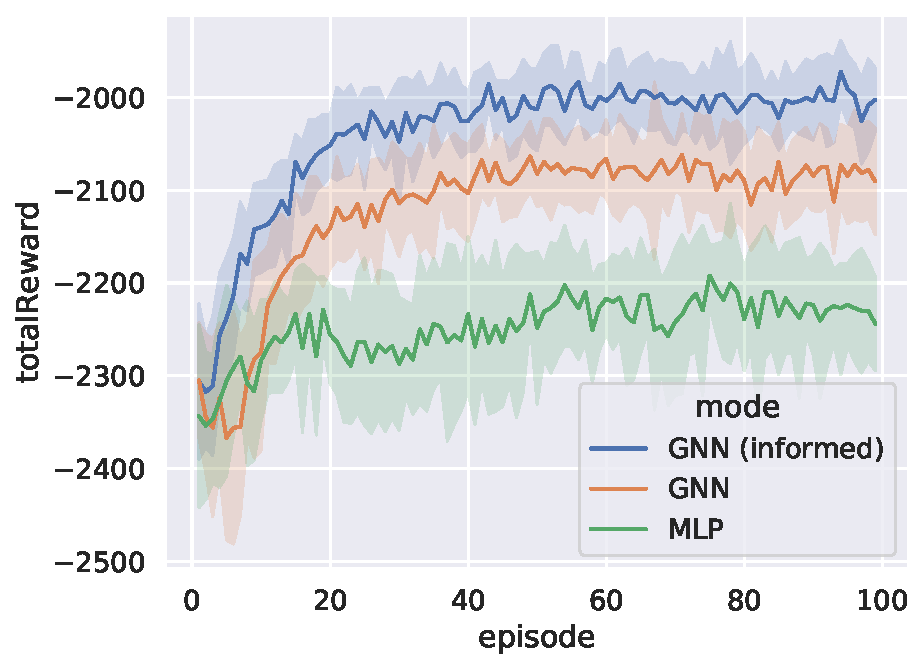
\includegraphics[width=0.36\textwidth]{img/reward-in-time.pdf}
\end{center}
\begin{center}
  \fbox{
  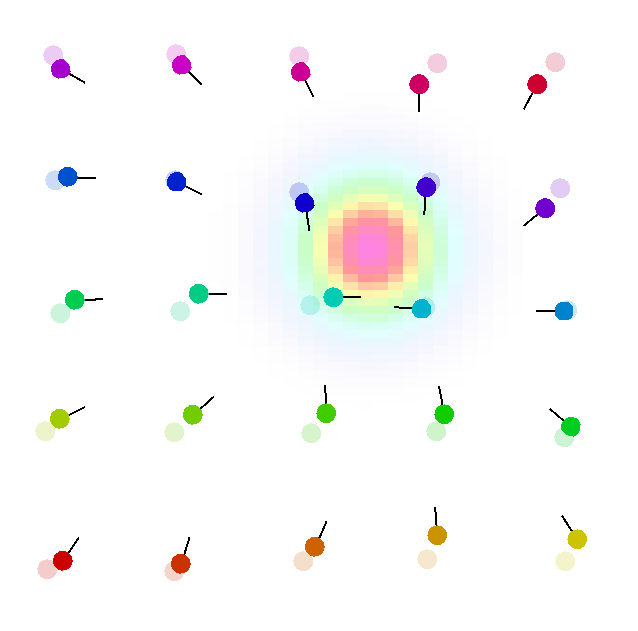
\includegraphics[width=0.25\textwidth]{img/start.png}
  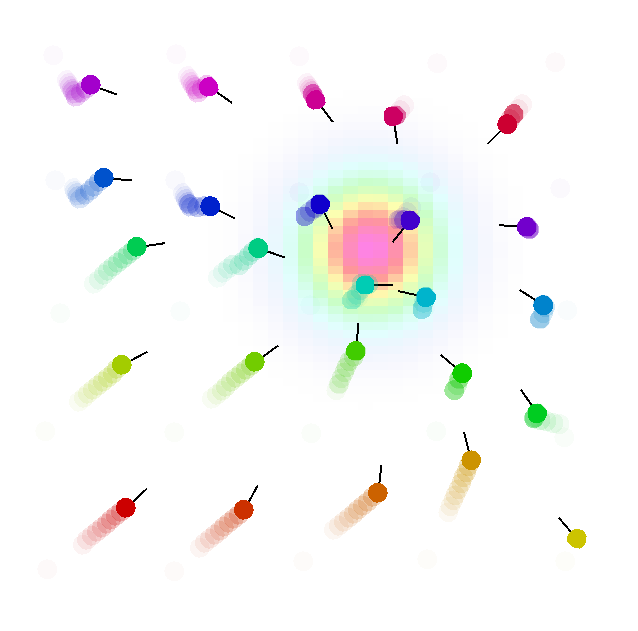
\includegraphics[width=0.25\textwidth]{img/after.png}
  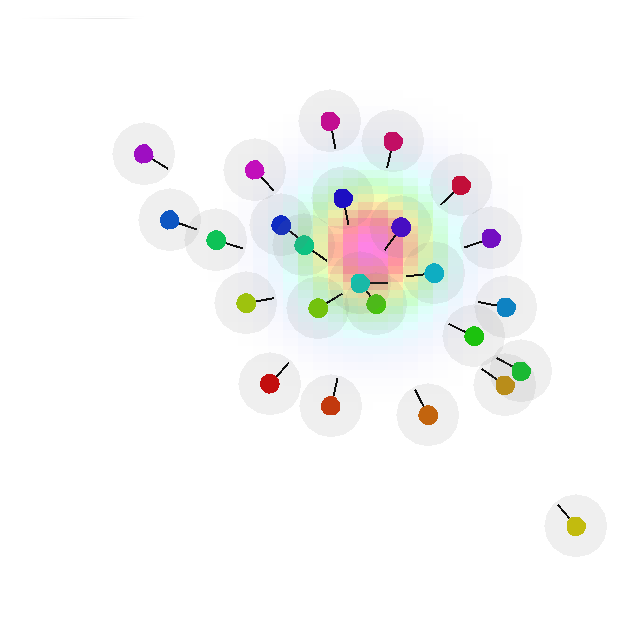
\includegraphics[width=0.25\textwidth]{img/end.png}}
  \end{center}
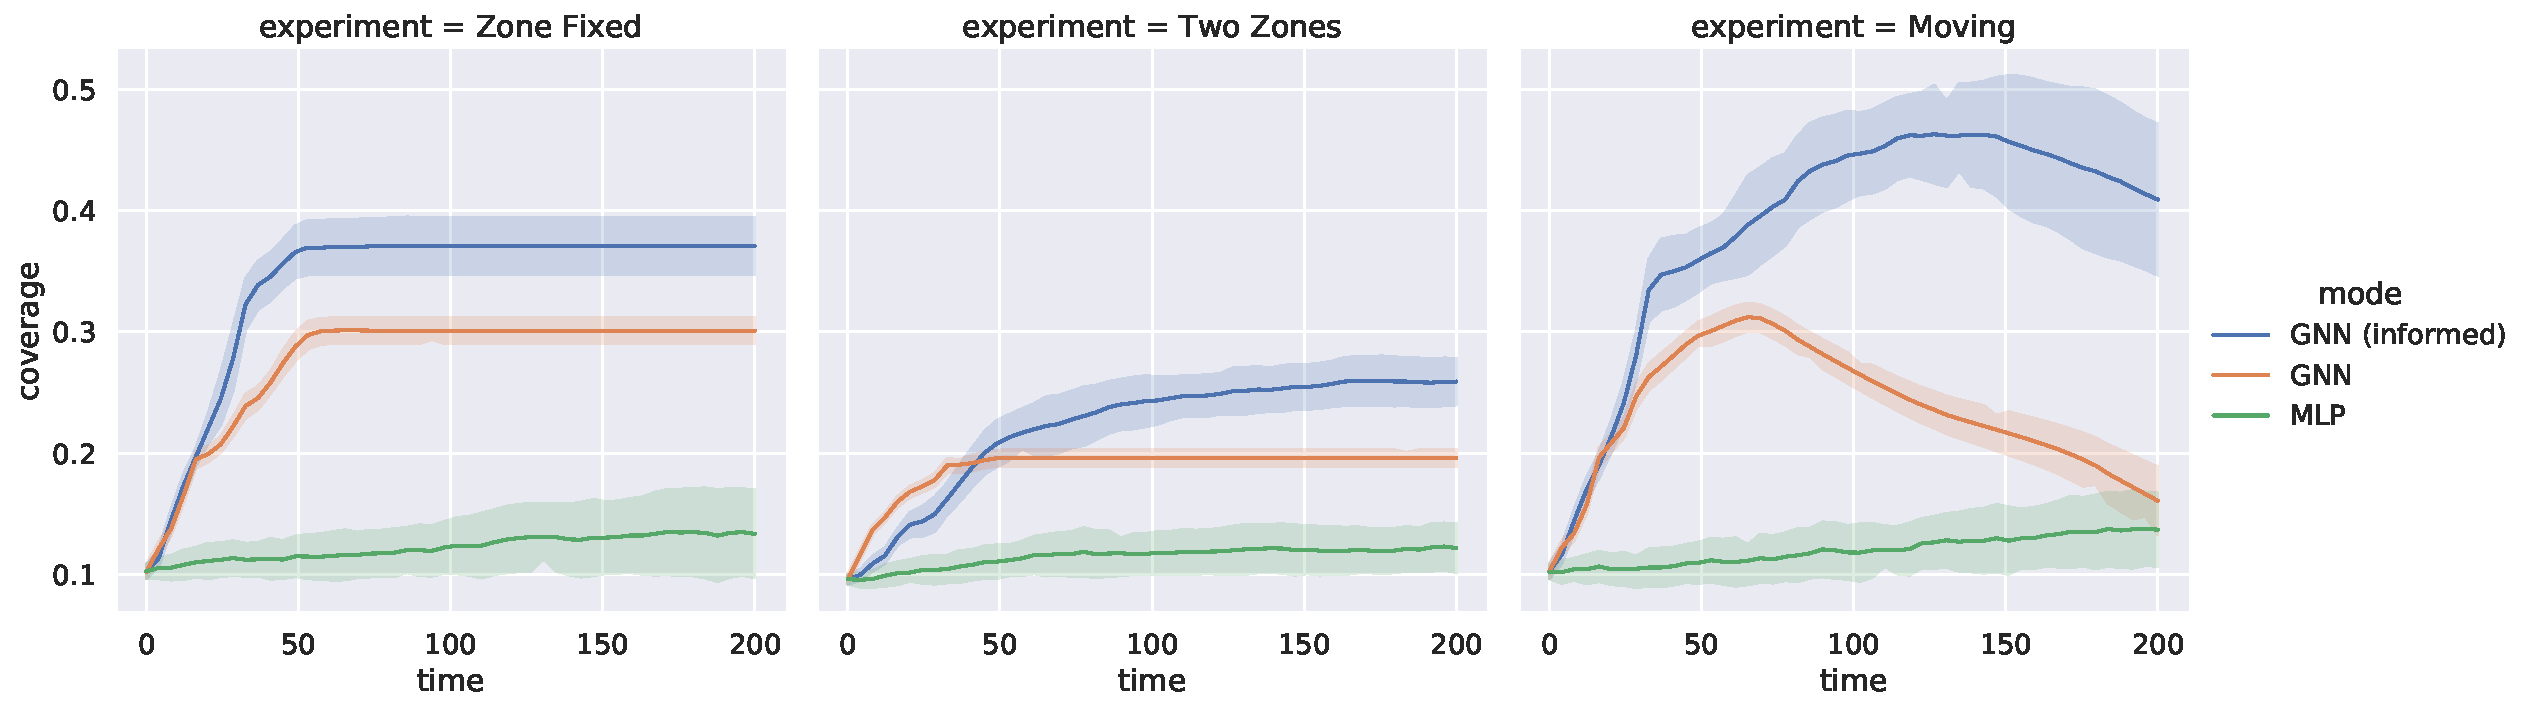
\includegraphics[width=\textwidth]{img/coverage-test.pdf}
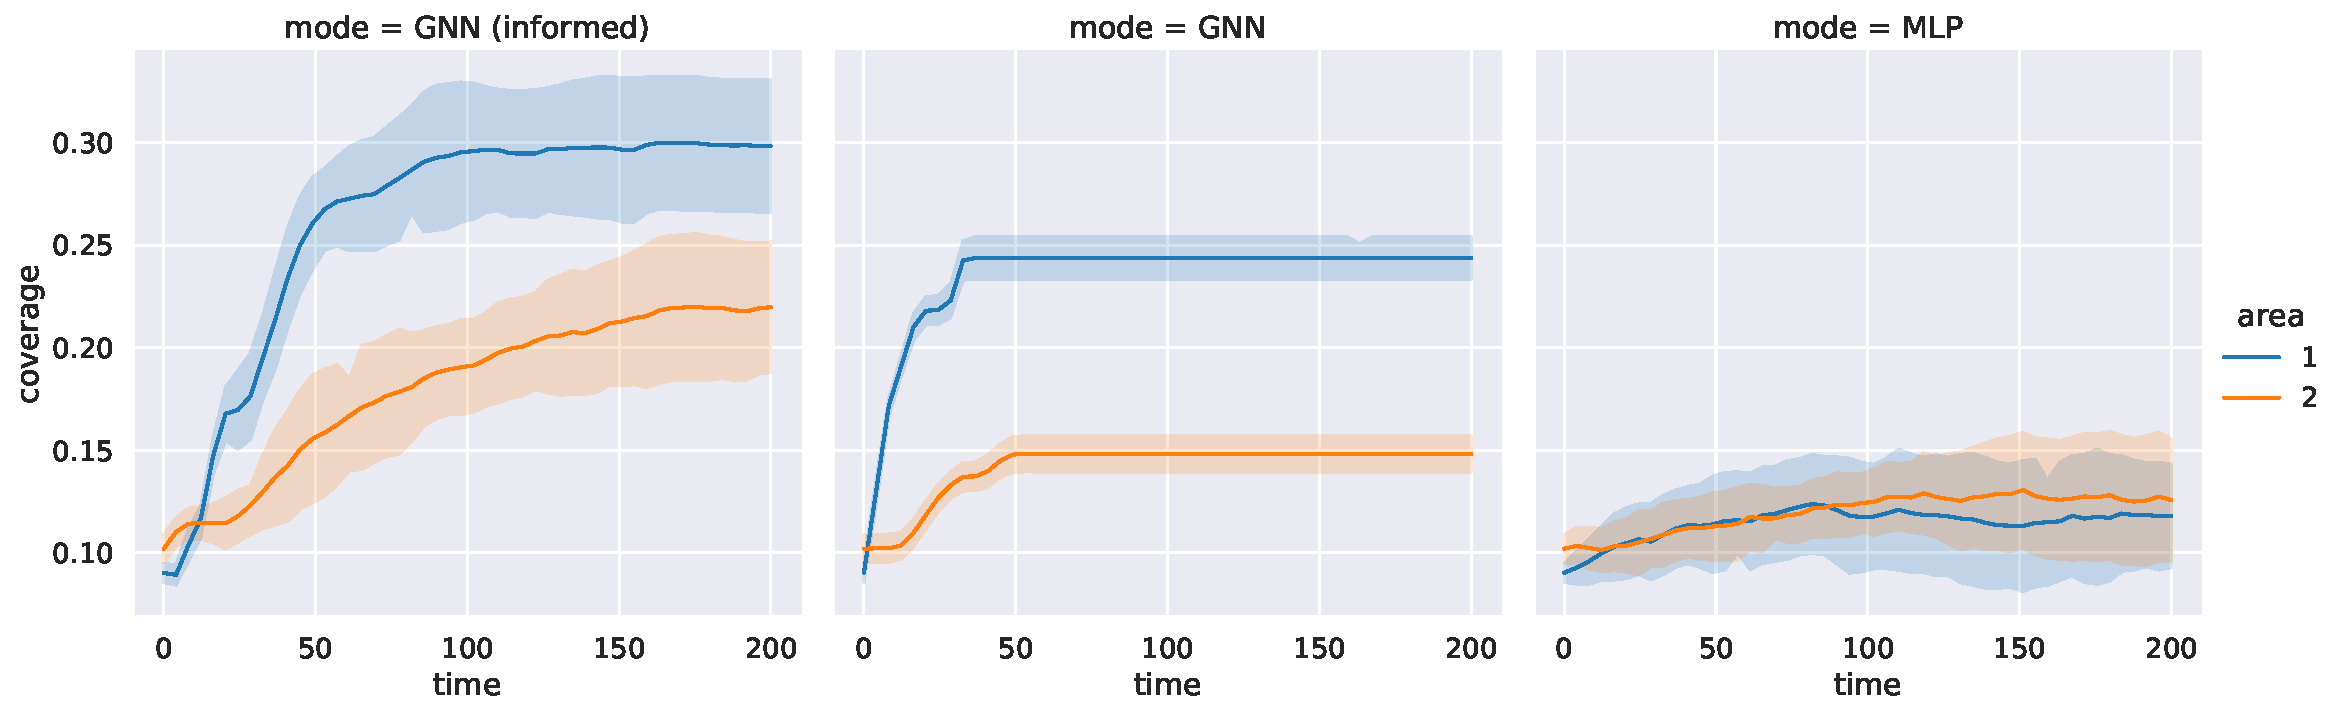
\includegraphics[width=0.92\textwidth]{img/coverage-two-test.pdf}

\end{frame}
\begin{frame}[fragile]{Engineering Methodologies}
  \bold{Areas of Improvement:}

  \begin{enumerate}
  \item \textbf{Programming Models \& APIs:}
  
  \begin{itemize}
  \item \textbf{FRASP~\cite{frasp}:} Functional reactive approach for self-organization programming (distributed, inspired by functional reactive programming).
  \item \textbf{MacroSwarm~\cite{macroswarm}:} API for expressing and composing swarm behaviors (extensive, covers various behaviors like aggregation and flocking).
  \end{itemize}
  
  \item \textbf{Distributed Sensing Deployment:}
  
  \begin{itemize}
  \item \textbf{Swarm Sensing API~\cite{swarm-clustering}:} Distributed and fault-tolerant clustering based on spatial-phenomena.
  \item \textbf{High-Level Abstractions for Distributed Sensing~\cite{aguzzi2022dynamic}:} Distributed and fault-tolerant sensing.
  \item \textbf{Pulverised Architecture:~\cite{aguzzi2021towards}} Opportunistic deployment of aggregate programs.
  \end{itemize}
  
  \item \textbf{DevOps; Continuous Integration:}
  
  \begin{itemize}
  \item \textbf{DevOps for CPSW~\cite{casadei2022towards}:} Continuous integration of software and physical parts of the system.
  \end{itemize}
  
  \end{enumerate}

  \bold{Tools:}
  
  \begin{itemize}
  \item \textbf{ScaRLib~\cite{domini2023scarlib}:} Cooperative multi-agent reinforcement learning tool (supports various learning schemes, integrates with PyTorch).
  \item \textbf{ScaFi-Web~\cite{aguzzi2021scafi}:} Web-based simulator for aggregate computing (useful for teaching and prototyping).
  \end{itemize}
  
\end{frame}
\begin{frame}[fragile]{MacroSwarm -- Overview}
\large{
A high-level\footnote{\tiny\fullcite{macroswarm}} compositional framework for expressing and composing swarm behaviors
}
\begin{center}
  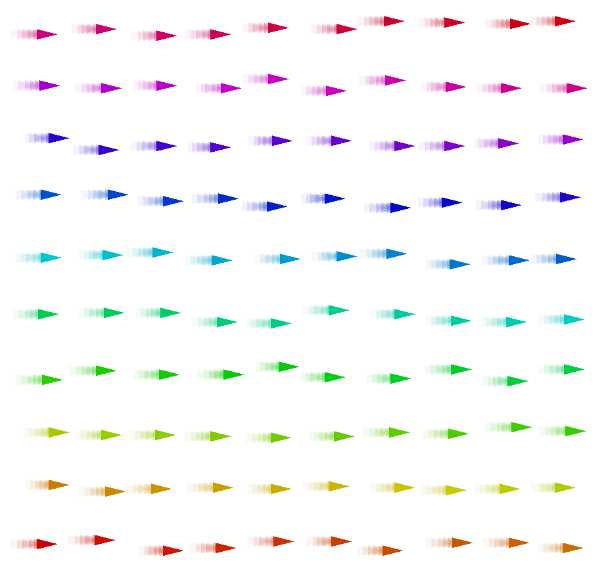
\includegraphics[height=2cm]{img/constant-movement.png}
  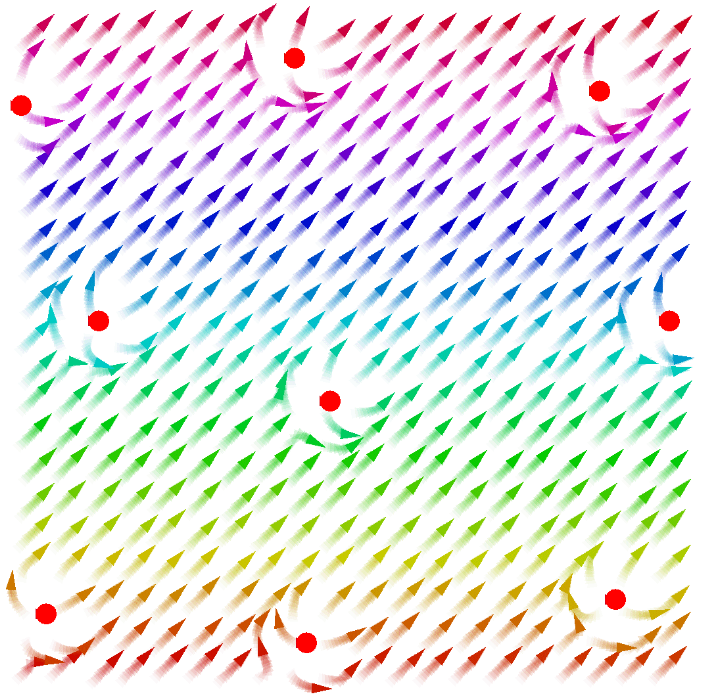
\includegraphics[height=2cm]{img/obstracle.png}		
  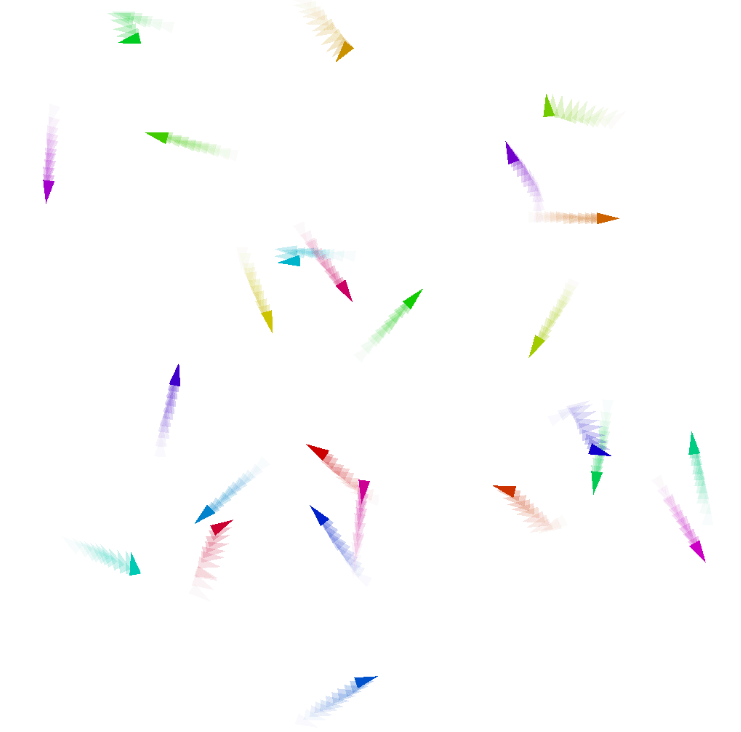
\includegraphics[height=2cm]{img/explore-2.png}
  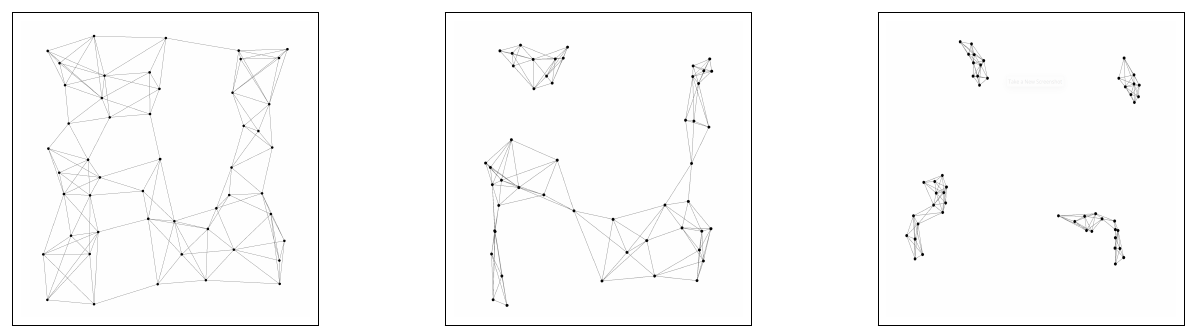
\includegraphics[height=2cm]{img/flock.png}
\end{center}
\begin{center}
  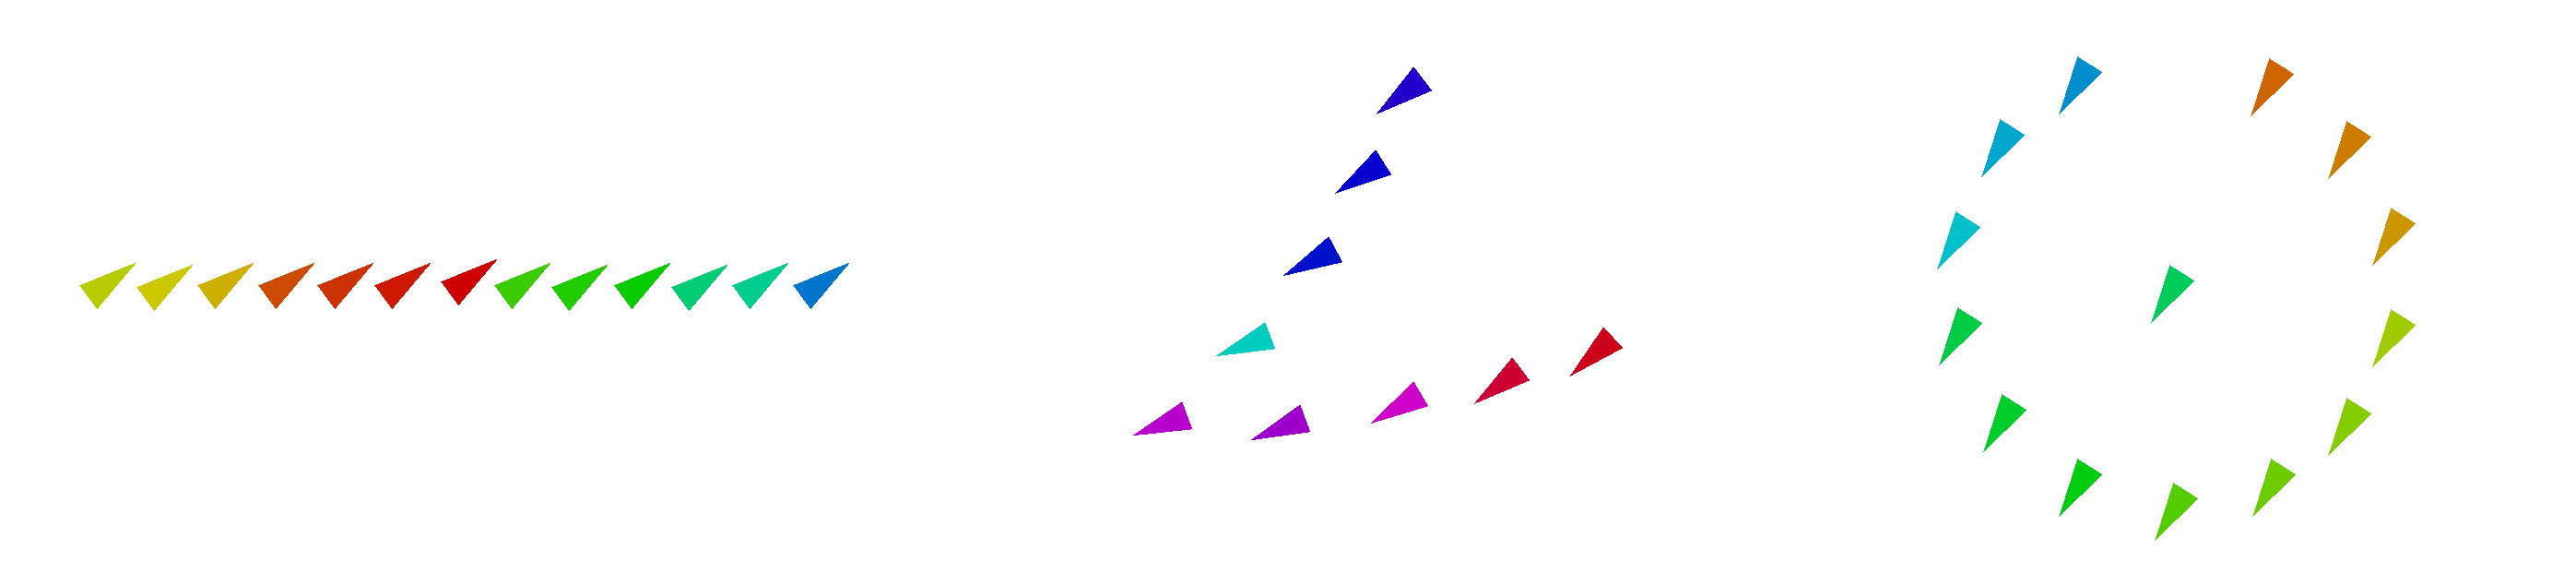
\includegraphics[height=1.5cm]{img/shapes.png}
\end{center}
\begin{center}
  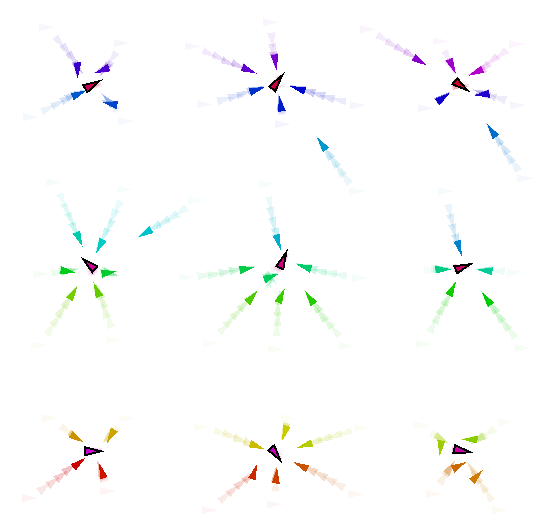
\includegraphics[height=2.3cm]{img/team-formation.png}
  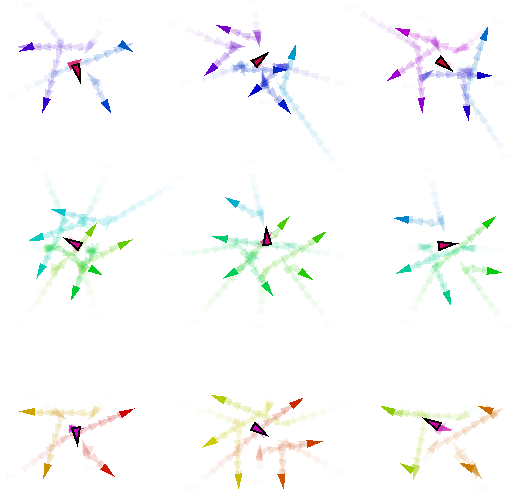
\includegraphics[height=2.3cm]{img/circle-formation.png}
  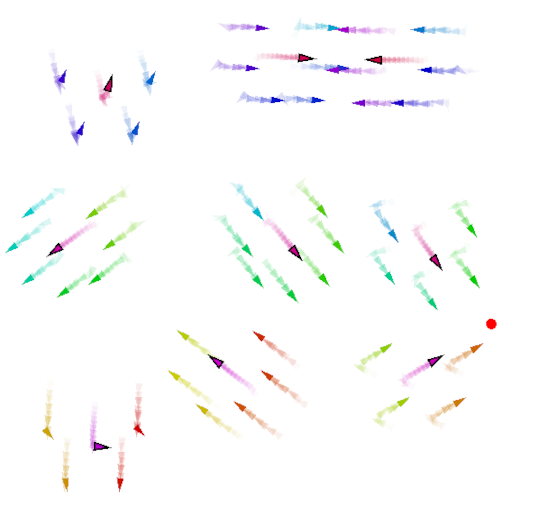
\includegraphics[height=2.3cm]{img/explore.png}
\end{center}
\end{frame}
\begin{frame}{Conclusion and Future Works}
\begin{itemize}
  \item This thesis discusses a novel approach to the engineering of CPSW application
  \item This poses the basis for a \emph{\underline{language-based}} approach to CPSW, putting together:
  \begin{itemize}
    \item \emph{\underline{Learning}}: Field-informed reinforcement learning, collective program sketching, distributed schedulers
    \item \emph{\underline{Tools}}: ScaFi, ScaRLib, ScaFi-Web
    \item \emph{\underline{Methodologies}}: FRASP, MacroSwarm, Swarm-Sensing API
  \end{itemize}
  \item Future works:
  \begin{itemize}
    \item Close the reality gap: deploy the aggregate programs on real CPSW, improve the toolchain, leverage realistic simulators (Gazebo, etc)
    \item Improve the learning algorithms: learn to deploy, learn to adjust runtime execution, etc.
    \item AC for learning: aggregate computing as a way create resilient infrastructure for learning (e.g., federated learning)
  \end{itemize}
\end{itemize}
\end{frame}

\begin{frame}
\centering{
  \Huge{Thank you!}
}
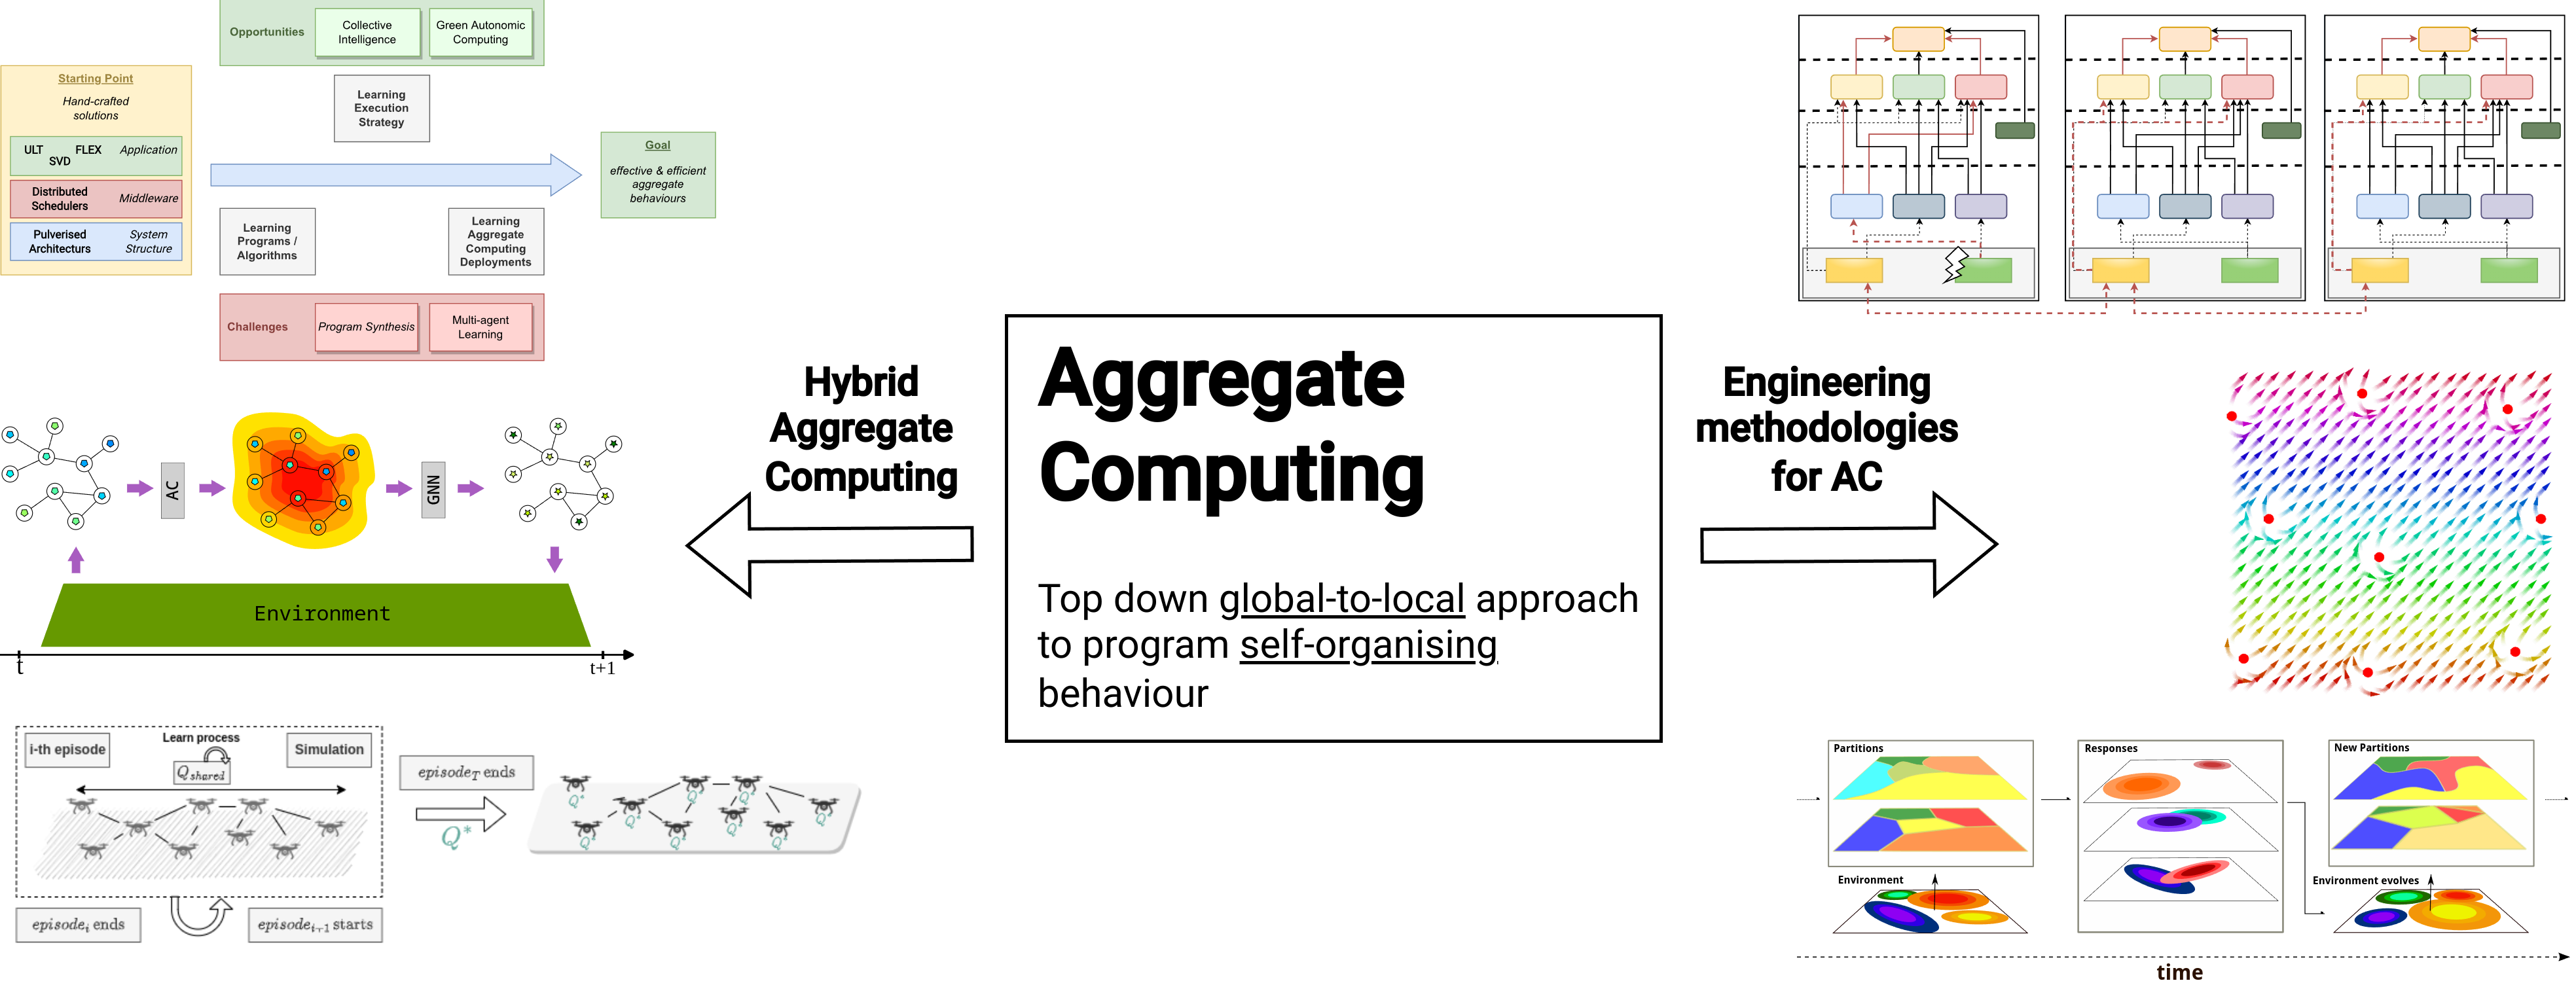
\includegraphics[width=\textwidth]{img/contribution.drawio.png}
\end{frame}
\begin{frame}[allowframebreaks]{References}
  \def\bibfont{\footnotesize}
  \printbibliography
\end{frame}

%%%%%%%%%%%%%%%%%%%%%%%%%%%%%%%%%%%%%%%%%%%%%%%%%%%%%%%%%%%%%%%%%%%%%%%%%%%%%%%%
\end{document}
%%%%%%%%%%%%%%%%%%%%%%%%%%%%%%%%%%%%%%%%%%%%%%%%%%%%%%%%%%%%%%%%%%%%%%%%%%%%%%%%

